%!TEX root = ../Thesis.tex
\section{Evaluierung verschiedener Arten der Einbindung von Microfrontends}\label{sec:Evaluierung}

In diesem Kapitel werden Kriterien festgelegt, anhand derer Arten der Einbindung von Microfrontends in die Portalshell bewertet und verglichen werden können. Dies geschieht durch eine Nutzwertanalyse, deren theoretische Grundlagen zunächst im nachfolgenden \cref{sec:TheoretischeGrundlagenEinerEvaluierung} erläutert werden. 

Anschließend werden in den \crefrange{sec:KriterienArtenEinbindung}{sec:VergleichDerArten} die vier relevanten Schritte einer Nutzwertanalyse am Thema durchlaufen: Identifizieren der Kriterien, Gewichten der Kriterien, Nutzwerte je Alternative bestimmen und Nutzwerte untereinander vergleichen.

Im letzten \cref{sec:OptimaleAnwendungsszenarien} werden die Ergebnisse der Nutzwertanalyse interpretiert und auf Anwendungsszenarien übertragen.

\subsection{Theoretische Grundlagen einer Nutzwertanalyse}\label{sec:TheoretischeGrundlagenEinerEvaluierung}

In diesem Abschnitt werden die theoretischen Grundlagen einer Nutzwertanalyse erläutert, welche in den nachfolgenden Abschnitten des \cref{sec:Evaluierung} angewendet werden, damit ein Entscheidungsproblem zwischen mehreren Auswahlalternativen fundiert gelöst werden kann.

Nach Christof Zangemeister ist die Definition einer Nutzwertanalyse \enquote{Die Analyse einer Menge komplexer Handlungsalternativen mit dem Zweck, die Elemente dieser Menge entsprechend der Präferenzen des Entscheidungsträgers bezüglich eines multidimensionalen Zielsystems zu ordnen. Die Abbildung dieser Ordnung erfolgt durch die Angabe der Nutzwerte (Gesamtwerte) der Alternativen.}\footnote{\cite[][45]{Zangemeister1971}}

In der Theorie nach Arnim Bechmann besteht die Nutzwertanalyse im Detail aus zehn Arbeitsschritten, welche nachfolgend in \cref{tab:NutzwertanalyseSchritte} dargestellt sind.

\newpage
\begin{table}[hbt]
	\centering
	\begin{minipage}[t]{1\textwidth}		
		\caption{Arbeitsschritte einer Nutzwertanalyse}
		\begin{tabularx}{\columnwidth}{|r|X|}
			\toprule
			Nr & Schritt \\
			\midrule
			1 & Problemformulierung\\
			2 & Aufstellung des Zielsystems\\
			3 & Angabe der zu bewertenden Alternativen $A_1,...,A_m$ \\
			4 & Bestimmung der Bewertungskriterien $K_1,...,K_n$ aufgrund des Zielsystems und der (Objekt-) Alternativen\\
			5 & Messung der Zielerträge $k_{11},...,k_{ij},...,k_{nm}$\\
			6 & Skalierung der Zielerträge in die Zielerfüllungsgrade $e_{11},...,e_{ij},...,e_{nm}$\\
			7 & Festlegung der Kriteriengewichte $g_1,...,g_n$\\
			8 & Berechnung der Teilnutzen $N_{ij}$ nach der Formel dargestellt in \cref{eq:NutzwertanalyseTeilnutzen}\\
			9 & Addition der Teilnutzen einer Alternative zum Nutzwert $N_j$ dieser Alternative\\
			10 & Angabe der Rangordnung der Alternativen aufgrund der Nutzwerte\\
			\bottomrule
		\end{tabularx}
		\source{\cite[Eigene Darstellung in Anlehnung an][28\psq]{Bechmann1978}}
		\label{tab:NutzwertanalyseSchritte}
	\end{minipage}
\end{table}

In der nachfolgenden \cref{eq:NutzwertanalyseTeilnutzen} ist die Formel zur Berechnung der Teilnutzwerte aus dem achten Schritt der vorherigen Tabelle zu sehen.

\begin{align*}
&\qquad\qquad\qquad\qquad\qquad N_{ij}=g_i \cdot e_{ij}\numberthis \label{eq:NutzwertanalyseTeilnutzen}\\ % Hack with \qquad
N_{ij} &= \textmd{Teilnutzen des i-ten Kriteriums der j-ten Alternative}\\
g_i &= \textmd{Gewichtung des i-ten Kriteriums}\\
e_{ij} &= \textmd{Zielerfüllungsgrad des i-ten Kriteriums der j-ten Alternative}
\end{align*}

Die zehn Schritte aus \cref{tab:NutzwertanalyseSchritte} sind in einem Ablaufschema in der nachfolgenden \cref{fig:NutzwertanalyseVorgehenBechmann} dargestellt. Das Ablaufschema stellt die Zusammenhänge der Einflussfaktoren zum Ergebnis, in diesem Fall die Nutzwerte, dar.

\newpage
\begin{figure}[hbt!]
	\centering
	\begin{minipage}[t]{0.7\textwidth}	
		\caption{Allgemeines Ablaufschema einer Nutzwertanalyse}
		\frame{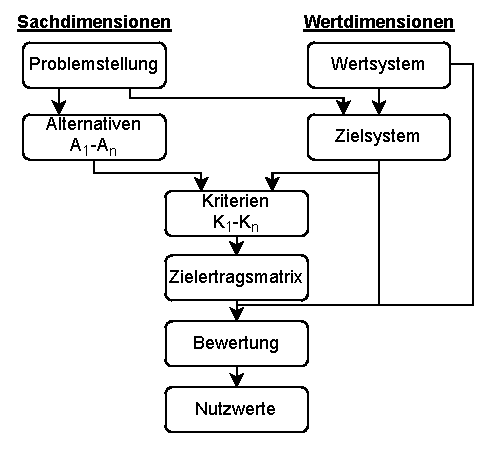
\includegraphics[width=1\textwidth]{img/NutzwertanalyseVorgehenBechmann}}\\ % Pfad
		\source{\cite[Eigene Darstellung in Anlehnung an][27]{Bechmann1978}} % Quelle
		\label{fig:NutzwertanalyseVorgehenBechmann}
	\end{minipage}
\end{figure}

Neben der Problemstellung und der für eine Nutzwertanalyse erforderlichen Lösungsalternativen fließen ebenfalls Entscheidungsregeln und Vorlieben des Autors als Wertesystem, sowie die Vorstellungen vom Zielsystem mit in die Bewertung ein.\footnote{\cite[vgl.][22\psq]{Bechmann1978}}

\enquote{Die zu bewertenden Alternativen werden bezüglich dieses Zielsystems durch Bewertungskriterien beschrieben.}\footnote{\cite[][26]{Bechmann1978}} Die Kriterien werden untereinander anhand ihrer Bedeutung gewichtet, damit wichtigere Kriterien mit höherem Anteil in den Nutzwert eingehen.

Die Gewichtung der Kriterien erfolgt durch die Paarvergleichsmethode. Jeder Teilnehmer der Nutzwertanalyse vergleicht jedes Kriterium gegeneinander. Es muss beim direkten Vergleich immer eine Entscheidung getroffen werden, welches Kriterium der beiden Verglichenen wichtiger ist. Zwei Kriterien dürfen nicht als gleich wichtig gesehen werden.\footnote{\cite[vgl.][15]{Kühnapfel2021b}}

Jeder Teilnehmer hat anschließend die Hälfte der nach der Gaußschen Summenformel (siehe nachfolgende \cref{eq:kleinerGauss}) errechneten Vergleiche durchgeführt, wobei \textit{N} für die Anzahl der Kriterien steht. Es wird nur die Hälfte durchgeführt, weil sich die andere Hälfte der Vergleiche automatisch bedingt. Denn ist \gls{K1} besser als \gls{K2}, so ist \gls{K2} zwangsläufig schlechter als \gls{K1}.

\begin{align*}
	&\,\, \sum_{k=1}^Nk=\frac{N}{2}(N+1) \numberthis \label{eq:kleinerGauss}\\ % Hack with \qquad
	N &= \textmd{Anzahl Kriterien}\\
\end{align*}

Die Summe aller individuellen Vergleiche wird anschließend in einer Vergleichsmatrix zusammengetragen, wie in der nachfolgenden \cref{fig:Praeferenzmatrix} dargestellt. Für jedes Kriterium kann nun die Gesamtsumme der gewonnenen Vergleiche errechnet werden.

\begin{figure}[hbt!]
	\centering
	\begin{minipage}[t]{0.85\textwidth}	
		\caption{Befüllte Präferenzmatrix mit Ergebnissen dreier Teilnehmer}
		\includegraphics[width=1\textwidth]{img/Präferenzmatrix}\\ % Pfad
		\source{\cite[Eigene Darstellung in Anlehnung an][194]{Schierenbeck2016}} % Quelle
		\label{fig:Praeferenzmatrix}
	\end{minipage}
\end{figure}

Aus der Summe der gewonnen Vergleiche je Kriterium wird anschließend der Rang jedes Kriteriums bestimmt. Das Kriterium, welches die meisten Paarvergleiche gewonnen hat, hat den höchsten Rang 1. Das Kriterium, welches die wenigsten Paarvergleiche gewonnen hat, bekommt den niedrigsten Rang N, welcher der Anzahl der Kriterien entspricht. Aus dem Rang kann der inverse Rang ermittelt werden, wie in der nachfolgenden \cref{eq:InverserRang} dargestellt ist.

\begin{align*}
&\qquad\qquad I_j=N + 1 - R_j \numberthis \label{eq:InverserRang}\\ % Hack with \qquad
I_j &= \textmd{Inverser Rang des j-ten Kriteriums}\\
N &= \textmd{Anzahl Kriterien}\\
R_j &= \textmd{Rang des j-ten Kriteriums}
\end{align*}

Aus dem inversen Rang wird anschließend das relative Gewicht jedes Kriteriums mit der nachfolgenden \cref{eq:RelativesGewicht} 
bestimmt.
\begin{align*}
&\qquad\qquad\qquad g_j=\frac{I_j}{\sum_{i=1}^NI_i} \numberthis \label{eq:RelativesGewicht}\\ % Hack with \qquad
g_j &= \textmd{Relatives Gewicht des j-ten Kriteriums}\\
N &= \textmd{Anzahl Kriterien}\\
I_j &= \textmd{Inverser Rang des j-ten Kriteriums}
\end{align*}

Dadurch erhält jedes Kriterium ein relatives Gewicht, welches in der nachfolgenden Nutzwertanalyse zur Gewichtung der Zielerfüllungsgrade genutzt werden kann. Sind alle Kriterien bekannt und gewichtet, so können die Teilnutzwerte der zu vergleichenden Alternativen bestimmt werden. In der nachfolgenden \cref{fig:RechenschemaNutzwertanalyse} ist die Durchführung einer Nutzwertanalyse dargestellt.

\begin{figure}[hbt!]
	\begin{minipage}[t]{1\textwidth}	
		\caption{Rechenschema einer Nutzwertanalyse}
		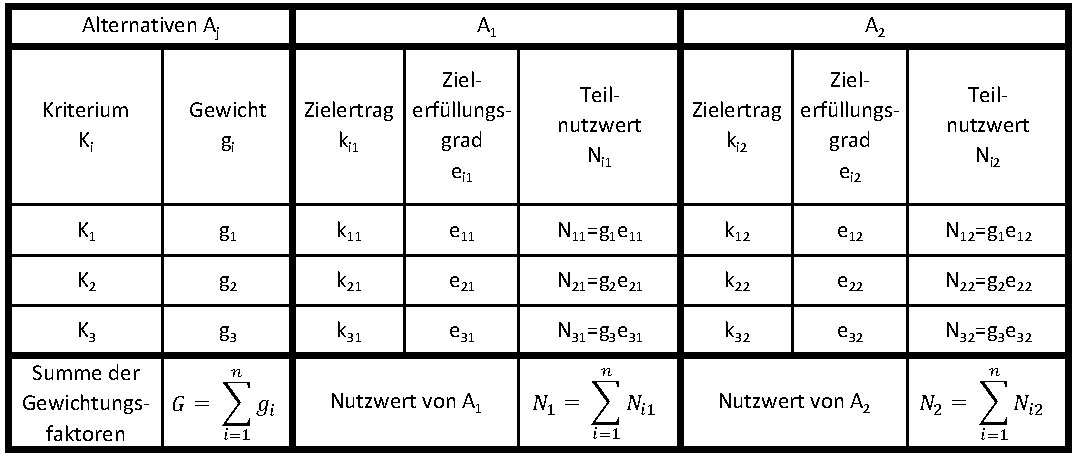
\includegraphics[width=1\textwidth]{img/Rechenschema}\\ % Pfad
		\source{\cite[Eigene Darstellung in Anlehnung an][30]{Bechmann1978}} % Quelle
		\label{fig:RechenschemaNutzwertanalyse}
	\end{minipage}
\end{figure}

Für jede Alternative $A_1$ bis $A_n$ wird der Zielertrag $k_{ij}$ des i-ten Kriteriums der j-ten Alternative bestimmt. Der Zielerfüllungsgrad $e_{ij}$ wandelt den ordinal messbaren Zielertrag jedes i-ten Kriteriums jeder j-ten Alternative in einen kardinal messbaren Wert um.\footnote{\cite[vgl.][29]{Bechmann1978}}  Die Skala der Zielerfüllungsgrade kann nach eigenem Ermessen bestimmt werden und kann beispielsweise von eins bis fünf oder eins bis zehn Punkten reichen.

Wird das Gewicht $g_i$ jedes i-ten Kriteriums mit dem Zielerfüllungsgrad $e_{ij}$ jedes i-ten Kriteriums jeder j-ten Alternative multipliziert, so erhält man den Teilnutzwert $N_{ij}$ jedes i-ten Kriteriums jeder j-ten Alternative. Die Summe aller Teilnutzwerte einer Alternative j ergibt den Nutzwert $N_j$.\footnote{\cite[vgl.][29]{Bechmann1978}}

Wenn dieses Vorgehen für alle j Alternativen wiederholt wird, so ist die Alternative mit dem höchsten Nutzwert die am besten geeignetste Alternative für die gegebene Ausgangsfragestellung.

\subsection{Kriterien für verschiedene Arten der Einbindung}\label{sec:KriterienArtenEinbindung}

In diesem Abschnitt werden die Kriterien definiert, anhand derer im \cref{sec:AnalyseVerschiedenerIntegrationsansaetze} die Arten der Einbindung von Microfrontends bewertet werden.

Ein Kriterium muss, damit es bewert- und vergleichbar ist, messbar sein. Einige Kriterien sind direkt messbar (kardinal), bspw. durch physikalische Größen. Andere Kriterien sind nicht direkt messbar (ordinal), weswegen bei diesen eine Punktevergabe stattfindet, um die ordinale Messbarkeit kardinal messbar zu machen und eine Vergabe von Zielerträgen zu ermöglichen.

Die Punkte für Kriterien werden auf einer Skala von 1 bis 5 vergeben. Ergebnisse von direkt messbaren Kriterien werden miteinander verglichen, nach Optimierungen untersucht und anschließend ebenfalls in einen Punktwert auf der Skala von 1 bis 5 Punkten umgerechnet. Ein Punkt bedeutet, dass das Kriterium nicht erfüllt wurde. Fünf Punkte bedeuten, dass das Kriterium maximal erfüllt wurde. Drei Punkte stehen für eine teilweise Erfüllung. Zwei Punkte für eine geringe und vier Punkte für eine gute Erfüllung.

Nachfolgend werden die Kriterien \textit{Übertragene Datenmenge}, \textit{Renderingzeit}, \textit{Entwicklungsaufwand}, \textit{Wartbarkeit}, \textit{Nähe am Standard}, \textit{Verschiedene Frameworks}, \textit{Kompatibilität}, \textit{Autonomie}, \textit{Unabhängigkeit der Entwicklerteams}, \textit{Lock-In Effekt} und \textit{Interoperabilität} erläutert. 

Die Kriterien entstammen zwei Expertengesprächen, welche im Rahmen der Nutzwertanalyse durchgeführt wurden. Die Protokolle der Gespräche sind in Anhang \ref{app:Expertengespräche} in den \Cref{Exp1,Exp2} nachzulesen.

\textbf{Übertragene Datenmenge}\\
Wenn Microfrontends eingebunden werden, müssen die zur Anzeige benötigten Dateien vom Server oder \gls{CDN} zum Client geladen werden. Je nachdem, mit welcher Art der Einbindung dies geschieht, variiert die Datenmenge. Eine größere Datenmenge die geladen werden muss, bedeutet eine längere Ladezeit bis zur Darstellung des Inhaltes, was besonders bei langsamen Internetverbindungen der Nutzer zu langen initialen Ladezeiten führen kann.

Die Datenmenge der Übertragung kann in Bytes gemessen werden. Die Menge variiert durch die Technologie der Komprimierung, ob Frameworks und Bibliotheken geteilt oder gecached werden und ob die Zusammensetzung der einzelnen Microfrontends serverseitig oder am Client passiert.

Die übertragene Datenmenge ist messbar, wenn der gleiche Inhalt eines Microfrontends bei mehrere Arten der Einbindung verglichen wird. Abzugrenzen ist die Datenmenge, welche der Portalshell zugehörig ist und nicht mit der Art der Einbindung in Verbindung gebracht wird. Die Datenmenge ist besonders relevant, wenn mehrere gleiche Microfrontends nebeneinander eingebunden werden. Im besten Fall skaliert die Datenmenge nicht linear mit den eingebundenen Microfrontends mit, sondern bleibt gleich.

\textbf{Renderingzeit}\\
Die Renderingzeit beschreibt die Zeit, welche vom Aufrufen durch die Portalshell bis zur Anzeige der Microfrontends vergeht. Sie hängt unter anderem mit der übertragenen Datenmenge zusammen, ist aber ebenfalls von der verwendeten Technologie abhängig. Die im Hintergrund ablaufenden Prozesse der Einbindungsarten benötigen unterschiedlich viel Zeit bis zur Darstellung des Inhaltes. Es wird in den nachfolgenden Beispielen in \textit{Time to Usability} gemessen, also bis der gesamte Inhalt geladen und dargestellt wurde. Andere Messverfahren, wie \textit{\gls{TTFB}} oder \textit{\gls{TTFD}}, wurden im Rahmen der Thesis nicht betrachtet.

Damit eine Vergleichbarkeit gegeben ist, muss auch bei diesem Kriterium der Vergleich anhand des selben Inhalts in verschiedenen Arten der Einbindung getätigt werden. Die Messung der Renderingzeit findet in Millisekunden statt.

\textbf{Entwicklungsaufwand}\\
Der Entwicklungsaufwand beschreibt den nötigen Anpassungsbedarf an der Portalshell und den jeweiligen Microfrontends. Im besten Fall bedarf es keiner Anpassung auf beiden Seiten. Es fällt lediglich der Aufwand der einmaligen Einbindung des Microfrontends an. Weitere Einbindungen der gleichen Art verursachen keinen weiteren Aufwand.

Die Summe der Anpassungsaufwände, die an der Portalshell und den Microfrontends entstehen sowie die Aufwände für das einmalige Einbinden und mehrfache Einbinden werden addiert. Die Aufwände werden in Personentagen geschätzt und sind dadurch kardinal messbar.

\textbf{Wartbarkeit}\\
Die Wartbarkeit beschreibt den Aufwand, welcher erbracht werden muss, damit die Art der Einbindung auf Dauer weiterhin funktioniert. Aspekte, wie Häufigkeit von Updates oder nötige Konfigurationsänderungen, werden in der Bewertung berücksichtigt. Besonders bei hohem Entwicklungsaufwand ist Wartbarkeit wichtig. Ein langfristig geringerer Wartungsaufwand rechtfertigt einen initial höheren Entwicklungsaufwand. Die Wartbarkeit ist nicht direkt messbar, kann aber durch gesammelte Aspekte in Punkte umgerechnet werden.

\textbf{Nähe am Standard}\\
Wenn eine Lösung zur Einbindung eines Microfrontends nah am Standard der verwendeten Technologie ist, sind dadurch Risiken, wie bspw. Breaking Changes oder Empfehlung zu einer anderen Lösung unwahrscheinlich. Da die Portalapplikation auf Angular beruht, sollten die Arten der Einbindung Unterstützung durch und zugesicherte Kompatibilität mit dem Angular Framework haben. Wenn das Angular Entwicklerteam Empfehlungen aussprechen würde, eine Art der Einbindung bewusst nicht einzusetzen, würde dies zu Anpassungsaufwänden führen, weil die betroffenen Microfrontends umgebaut werden müssten.

Die Nähe zum Standard ist nicht direkt messbar, kann aber durch Vergleiche der jeweiligen Microfrontend Technologien untereinander und anhand bestehender Statements der Technologiehersteller der Portalshell verglichen werden. 

\textbf{Verschiedene Frameworks}\\
Die Unterstützung verschiedener Web Frameworks bedeutet mehr Flexibilität und Autonomie der Entwicklerteams. Die Angular Portalshell aus dem vorherigen Kapitel wird nicht auf ein anderes Framework migriert.\newline
Die Microfrontends verwenden jeweils nur ein Web Framework, diese können sich aber untereinander unterscheiden. Die Entwicklerteams müssen sich im besten Fall gar nicht gegenseitig abstimmen. Eine direkte Messung ist nicht möglich, allerdings kann eine Tendenz ermittelt werden und Abstufungen möglicher Technologien in verschiedenen Konstellationen festgehalten werden.

\textbf{Kompatibilität}\\
Die Kompatibilität beschreibt, wie gut sich die Art der Einbindung mit anderen Standards und Techniken kombinieren lässt. Eventuell müssen durch die Auswahl einer bestimmten Art der Einbindung einige Features der Portalshell oder der Microfrontends aus- oder umgebaut werden. Eine Liste an sich ausschließenden Verwendungen kann zur Bewertung herangezogen werden. Beispiele hierfür können Designframeworks sein, die miteinander nicht kompatibel sind oder es sind Features wie dynamisches Einbinden oder asynchrones Laden. 

\textbf{Autonomie}\\
Die Autonomie beschreibt, inwieweit das Microfrontend und die Portalshell unabhängig voneinander existieren können. Im besten Fall sind sowohl Microfrontend, als auch die Portalshell, unabhängig voneinander. Im schlechtesten Fall kann das Microfrontend nicht ohne Parameter oder geteilte Bereiche der Portalshell funktionieren. Zur Robustheit sollten die Microfrontends autonom funktionieren.

Auch die Autonomie ist nicht direkt messbar, kann aber ebenfalls durch begründete Aspekte in Punkte umgerechnet werden.

\textbf{Unabhängigkeit der Entwicklerteams}\\
Die Unabhängigkeit der Entwicklerteams beschreibt, wie sehr die Teams, welche an verschiedenen Microfrontends arbeiten, voneinander losgelöst agieren können. Im besten Fall kann jedes Team seine eigenen Entscheidungen treffen und es treten keine Seiteneffekte auf.\newline
Im schlechtesten Fall müssen jegliche Änderungen mit den anderen Entwicklerteams abgesprochen werden und eine autonome Arbeitsweise sowie individuelle Entscheidungsfindungen sind nicht möglich. So müssen sich eventuell Teams untereinander abstimmen, wie sie die gegenseitige Beeinflussung durch Styles und Performance unterbinden.

Dieses Kriterium ist nicht direkt messbar und muss ebenfalls in Punkte umgerechnet werden.

\textbf{Lock-In Effekt}\\
Der Lock-In Effekt beschreibt, wie stark man sich durch Verwendung dieser Art der Einbindung festsetzt. Wenn der initiale Aufwand zum Einrichten der Einbindungsart sehr hoch ist und anschließend der Aufwand zum Wechseln auf eine andere Art ebenfalls sehr hoch ist, besteht ein Lock-In Effekt. Der Lock-In Effekt ist nicht gegeben, wenn durch geringen Aufwand die Art der Einbindung gewechselt werden kann.

Es wird sowohl der Aufwand an der Portalshell, als auch der Aufwand an den Microfrontends bewertet. Ein Lock-In Effekt ist nicht klar definiert und kann daher in Abstufungen vorliegen, welche nicht kardinal messbar sind.

\textbf{Interoperabilität}\\
Die Interoperabilität beschreibt, wie gut Microfrontends durch die Art der Einbindung mit der Portalshell, aber auch anderen Microfrontends interagieren, und kommunizieren können. Zur Interoperabilität zählt das generelle Einbinden und Betreiben dieser Art. Dazu kommen Aspekte, welche sich auf Parameter- und Datenaustausch beziehen.

Bewertet werden können der Aufwand, welcher zum Einrichten von Datenübertragung nötig ist, welche Datentypen übertragen werden können, sowie die Flexibilität, welche die Schnittstellen aufbringen. Ebenfalls gibt es potentielle Konzepte der Kommunikation von Microfrontends untereinander.

Hohe Punktzahl erreichen Lösungen, die eine hohe Interoperabilität aufweisen, welche sich durch einfache, sichere und schnelle Kommunikation mit der Portalshell sowie anderen Microfrontends äußert.

\textbf{Zusammenfassung}\\
In der nachfolgenden \cref{tab:UebersichtKriterien} sind alle elf Kriterien noch einmal aufgelistet. Die Kriterien sind entweder objektiv messbar anhand von Einheiten oder subjektiver Natur, welche aber durch Begründungen und Nachweise belegt werden können.

\begin{table}[hbt]
	\centering
	\begin{minipage}[t]{1\textwidth}	
		\caption{Vergleichskriterien für Arten der Einbindung von Microfrontends}
		\begin{tabularx}{\columnwidth}{|cXX|}
			\toprule
			\textbf{Nr} & \textbf{Kriterium}	& \textbf{Messbar durch} \\
			\midrule
			1 & Übertragene Datenmenge & Differenz Bytes \\
			2 & Renderingzeit & Millisekunden \\
			3 & Entwicklungsaufwand & Personentage \\
			4 & Wartbarkeit & Subjektiv \\
			5 & Nähe am Standard & Subjektiv \\
			6 & Verschiedene Frameworks & Subjektiv \\
			7 & Kompatibilität & Subjektiv \\
			8 & Autonomie & Subjektiv \\
			9 & Unabhängigkeit der Entwicklerteams & Subjektiv \\
			10 & Lock-In Effekt & Subjektiv \\
			11 & Interoperabilität & Subjektiv \\
			\bottomrule
		\end{tabularx}
		\source{Eigene Darstellung}
		\label{tab:UebersichtKriterien}
	\end{minipage}
\end{table}

Die elf Kriterien der vorherigen Tabelle werden im nachfolgenden \cref{sec:GewichtenKriterien} gegeneinander nach Wichtigkeit sortiert und mit einem entsprechendem Gewicht versehen.

\subsection{Gewichtung der Kriterien}\label{sec:GewichtenKriterien}

In diesem Abschnitt wird die Gewichtung der Kriterien, welche im vorherigen \cref{sec:KriterienArtenEinbindung} aufgelistet wurden, nach dem Prozess der in \cref{sec:TheoretischeGrundlagenEinerEvaluierung} erklärten Paarvergleichsmethode vorgenommen.

Das Befüllen der Paarvergleichsmatrix wurde im Rahmen eines Expertengespräches mit fünf Teilnehmern durchgeführt. Die Teilnehmer haben seit mehreren Jahren Erfahrung im Umgang mit Portalapplikationen und setzen sich zusammen aus zwei Software-Architekten, zwei Software-Entwicklern und einem IT-Projektmanager.

Im Prozess des Befüllens der Präferenzmatrix haben alle Teilnehmer individuell jedes Kriterium miteinander vergleichen und dem wichtigeren Kriterium jeweils einen Punkt gegeben.

In der nachfolgenden \cref{fig:Paarvergleichsmethode} ist die ausgefüllte Paarvergleichsmatrix dargestellt, welche die Summe der fünf Einzelbewertungen enthält.

\begin{figure}[hbt!]
	\begin{minipage}[t]{1\textwidth}	
		\caption{Ausgefüllte Paarvergleichsmatrix}
		\includegraphics[width=1\textwidth]{img/AusgefüllteMatrix}\\ % Pfad
		\source{Eigene Darstellung} % Quelle
		\label{fig:Paarvergleichsmethode}
	\end{minipage}
\end{figure}

In der Tabelle ist zu sehen, dass das Kriterium \textit{Interoperabilität} in Summe 39 Punkte erhalten hat und damit knapp vor \textit{Wartbarkeit} mit 38 Punkten und \textit{Unabhängige Entwicklerteams} mit 35 Punkten liegt. 
Die Spalte Rang stellt die Rangfolge der Kriterien absteigend nach ihrer bewerteten Wichtigkeit dar. Anhand des Ranges konnte mit der \cref{eq:InverserRang} der inverse Rang I gebildet werden. Aus dem inversen Rang wurde für jedes Kriterium durch die \cref{eq:RelativesGewicht} das relative Gewicht G bestimmt.

Das wichtigste Kriterium \textit{Interoperabilität} hat somit ein relatives Gewicht von 16,67\% und das von den elf Kriterien am wenigsten wichtig bewertete Kriterium \textit{Datenmenge} wird nur mit 1,52\% gewichtet.

Mit den ermittelten Kriteriengewichten kann nun im nachfolgenden Schritt der Teilnutzwert jedes Kriteriums von jeder Art der Einbindung bestimmt werden.

\subsection{Analyse verschiedener Integrationsansätze}\label{sec:AnalyseVerschiedenerIntegrationsansaetze}

In diesem Abschnitt werden die zur Auswahl stehenden alternativen Arten der Einbindung von Microfrontends in eine Portalshell verglichen. Im nachfolgenden \cref{sec:Abgrenzung Ansaetze} werden dafür zunächst die nicht in Betracht gezogenen Alternativen begründet und abgegrenzt. 
In den darauffolgenden Abschnitten werden anschließend die zum Vergleich ausgewählten Alternativen im Detail für jedes Kriterium untersucht und die jeweilige Erfüllung festgehalten.

\subsubsection{Abgrenzung unpassender Ansätze}\label{sec:Abgrenzung Ansaetze}

Zu Beginn dieser Arbeit wurden in \cref{sec:Portalapplikationen}, \cref{sec:PortalapplikationenHyperlinks} und \cref{sec:Microfrontends} verschiedene Arten der Realisierung von Microfrontends und Portalapplikationen beschrieben.

Portalapplikationen bestehend aus Hyperlinks sind eine einfache Möglichkeit, eine Microfrontend-Architektur darzustellen. Zur Realisierung benötigt es lediglich eine einfache Webseite, welche zu jedem referenzierten Microfrontend einen Link enthält. Bezogen auf die Beispielapplikation aus dem vorherigen \cref{sec:PrototypischesBeispiel} können die Anforderungen in Bezug auf einheitliches Design und eingebundene, kaum spürbare Navigation nicht erfüllt werden. Durch das Klicken auf den Hyperlink wird entweder die gesamte Webseite gewechselt oder die angeklickte Seite öffnet sich in einem neuen Tab.\footnote{\cite[vgl.][]{Steyer2018}} Dieses Verhalten steht der Anforderung von softem Routing diametral entgegen. 

Ebenfalls ist das Übertragen von Parametern von der Portalapplikation zu den Microfrontends erschwert sowie eine Zugriffsbeschränkung auf Teilbereiche ebenfalls nur durch hohen Mehraufwand realisierbar.

Microfrontends durch serverseitiges Rendering sind ebenfalls keine passende Lösung, weil im prototypischem Beispiel eine Angular Portalapplikation gewählt wurde. Angular ist ein Frontend Framework für \gls{SPA}s zum clientseitigen Rendern, welches softes Routing ermöglicht.

In den nachfolgenden vier Abschnitten werden die vier grundlegend zutreffenden Ansätze \textit{Iframe}, \textit{Web Components}, \textit{Module Federation} und \textit{Module Federation mit Web Components} auf die Erfüllung der in \cref{sec:KriterienArtenEinbindung} definierten Kriterien untersucht.

Damit die Kriterienerfüllung vergleichbar ist, wurde für die vier Arten der Einbindung jeweils ein identisches Microfrontend erstellt und in eine prototypische Portalshell eingebunden.

Dieses vergleichbare Microfrontend ist exemplarisch für das Iframe in Anhang \ref{app:Bilder} in \cref{fig:EvalAnsicht} dargestellt. Für die anderen drei Arten der Einbindung wurde ein gleiches Microfrontend erstellt. Lediglich der Name der Einbindungsart in der Überschrift wurde entsprechend ausgetauscht. Die sich dadurch minimal unterscheidende Datenmenge durch mehr oder weniger übertragene Bytes ist zu vernachlässigen.

Das vergleichbare Microfrontend besteht aus einer Überschrift gestyled mit \gls{CSS}, einem Beispielbild sowie einer Angular Material Komponente, konkret einem animierten Fortschrittsbalken.

\subsubsection{Iframe}\label{sec:EvaluierungIFrame}

In diesem Abschnitt wird das Iframe als Microfrontend zur Einbindung in eine Portalshell bewertet. Für die Bewertung werden die im vorherigen \cref{sec:GewichtenKriterien} gewichteten Kriterien verwendet. Die nachfolgenden elf Kriterien sind absteigend nach ermittelten zugehörigen Gewichten sortiert.

Bei den nachfolgend kardinal messbaren Kriterien \textit{Entwicklungsaufwand} , \textit{Renderingzeit} und \textit{Übertragene Datenmenge} werden in diesem Abschnitt bereits die Messergebnisse der anderen drei Einbindungsarten vorweggenommen. Dadurch steht der ermittelte Zielerfüllungsgrad der Alternativen in direktem Vergleich zueinander. Die Begründung oder die Nachweise zum jeweiligen Zielertrag sind in den Abschnitten der Einbindungsarten zu finden.

\textbf{Interoperabilität}\\
Interoperabilität ist der größte Nachteil von Iframes. Der Datenaustausch zur Portalshell und zwischen den Microfrontends ist komplex.

Das Einbinden in die Portalshell ist einfach, solange keine Parameter übertragen werden müssen. Einfache Parameter können über den Querystring von der Portalshell in das Iframe Microfrontend übergeben werden. Dies funktioniert allerdings nur bei nicht sicherheitskritischen Parametern, wie bspw. dem Standort-Parameter einer Wetter-App, denn Parameter über einen Querystring zu übertragen ist nicht sicher und kann manipuliert werden.\footnote{\cite[vgl.][35]{Mezzalira2021}}

Wenn allerdings sicherheitskritische Parameter, die entweder persönliche Informationen enthalten oder nicht modifiziert werden dürfen, vorliegen, dann ist der Querystring nicht geeignet. Dies ist dadurch bedingt, dass der Querystring unter anderem von Administratoren geloggt, aber auch vom Anwender manipuliert werden kann.

Im Fall von informationskritischen Parametern oder benötigter Authentifizierung muss eine sicherere Möglichkeit gefunden werden, um die Parameter zu überreichen und den Anwender zu authentifizieren. Dies kann über gängige Authentifizierungsprotokolle, wie \gls{OIDC} oder \gls{SAML} abgebildet werden.

Im Fall von \gls{SAML} müsste eine Schnittstelle der Portalshell die zu übertragenden Informationen in einem \gls{SAML}-Token verschlüsseln und dann an eine am Microfrontend konfigurierte \gls{SAML}-Schnittstelle als POST-Request übertragen. Die Einbindung einer \gls{SAML}-Schnittstelle kann über eine vom Portalteam bereitgestellte Bibliothek geschehen, was sich aber wiederum negativ auf den initialen Entwicklungsaufwand sowie die Autonomie der Entwicklerteams auswirkt.

Wenn ein Benutzer mehrfach den gleichen Inhalt eines Iframe Microfrontends einbinden möchte, so muss er dies auch mehrfach tun. Iframes skalieren nicht in der Einbindung und teilen auch keine Bibliotheken untereinander oder mit der Portalshell. So kommt es auch zu mehrfachen Requests und die übertragene Datenmenge steigt ebenfalls mit der Anzahl der eingebundenen gleichen IFrames.

Aus diesen Gründen wird das Kriterium \textit{Interoperabilität} mit einer Gewichtung von 16,67\% mit 1 von 5 Punkten bewertet und erhält daher einen Teilnutzwert von 0,1667.

\textbf{Wartbarkeit}\\
Der Aufwand für Wartung bei einem Iframe ist überschaubar. Im Falle einer neuen Version des Microfrontends muss dieses neu veröffentlicht werden, was allerdings durch eine einmalig eingerichtete \gls{CI/CD} Pipeline automatisiert geschehen kann. 

Iframes sind unabhängig von den benutzten Frontend-Frameworks und -Technologien. Von daher sind keine regelmäßigen Updates zu erwarten, auch nicht, wenn sich die Frameworkversion beispielsweise durch ein Update von Angular 12 auf 13 erhöht. Lediglich bei einem Update der \gls{HTML}-Version könnten sich theoretisch Eigenschaften des Iframe-Tags verändern, was aber eher unwahrscheinlich ist.

Das Iframe referenziert ein gehostetes Microfrontend. Wenn eine neue Version des Microfrontends gleichzeitig zu einer Bestandsversion existieren soll, müssten zwei unterschiedliche Versionen des gleichen Microfrontends auf unterschiedlichen URLs gehostet werden. Dies kann beispielsweise bei einem Rollout der Fall sein, bei dem nur konfigurierte Betatester die neuste Version erhalten und Nicht-Betatester die Bestandsversion weiterhin verwenden. 

Dies kann beispielsweise über verschiedene URL-Routen der gleichen Domain realisiert werden. Das Portal muss in dem Fall wissen, für welche User es auf die jeweilige \gls{URL} weiterleiten muss. Ein ähnlicher Ansatz mit dem gleichen Ziel wäre das sogenannte \textit{Blue-Green Deployment}, bei welchem zwei Versionen des Microfrontends gleichzeitig gehostet werden und diese bei Bedarf die genutzte Route wechseln können.\footnote{Mehr Informationen über Blue-Green Deployment unter \cite[][]{CloudFoundryDocumentation2020}}

Ein weiterer negativer Aspekt ist, dass das ganze Microfrontend im Falle einer neuen Version neu veröffentlicht werden muss, was mit einer Ausfallzeit einhergeht.

Die \textit{Wartbarkeit} mit einer Gewichtung von 15,15\% wird mit 3 von 5 Punkten bewertet und erhält dadurch einen Teilnutzwert von 0,4545.

\textbf{Unabhängige Entwicklerteams}\\
Unabhängige Entwicklerteams können durch Iframes realisiert werden. Das Team, welches das Microfrontend betreut, ist grundsätzlich nicht auf andere Teams angewiesen. Es sei denn, man stimmt sich gegenseitig über Schnittstellen ab oder muss den Austausch von sicheren Parametern und Authentifizierung ermöglichen, wie vorher beim Kriterium \textit{Interoperabilität} beschrieben. In dem Fall müssen die zu übertragenden Parameter abgestimmt werden und eine Bibliothek des Portalteams eingebunden werden, die das Auslesen der Parameter übernimmt und die Authentifizierung durchführt.

Wenn das Microfrontendteam nicht in der gleichen Programmiersprache, wie das Portalteam entwickelt, muss das Portalteam eine Schnittstellendokumentation zur Verfügung stellen, anhand derer die Funktionen nachgebaut und die Parameter ausgelesen werden können.

Das Kriterium \textit{Unabhängige Entwicklerteams} mit einer Gewichtung von 13,64\% wird mit 4 von 5 Punkten bewertet, weil lediglich Abhängigkeit zwischen dem Portalteam und dem Microfrontendteam besteht, wenn Authentifizierung oder sicherer Parameteraustausch durchgeführt werden muss. Der Teilnutzwert des Kriteriums beträgt demnach 0,5456.

\textbf{Kompatibilität}\\
Das Iframe wird vollständig mit allem Seitenmarkup in dem \gls{DOM}-Tree der Portalapplikation eingebunden. Dadurch doppeln sich \gls{HTML} Elemente, wie zum Beispiel der Header. Screenreader und Crawler von Suchmaschinen sind durch diese Seitenstruktur häufig verwirrt und erzielen schlechte Resultate.\footnote{\cite[vgl.][]{GoogleSearchCentral2022}}

Ebenfalls weist das Iframe diverse Sicherheitslücken auf, die ausgenutzt werden können. So sind \textit{Iframe Phishing}, \textit{Clickjacking}, \textit{Cross-Frame Scripting} und \textit{Iframe Injection} Sicherheitsrisiken, welche Hacker auf Webseiten mit Iframes ausnutzen können.\footnote{\cite[vgl.][]{Gunawardhana2021}}

Positiv gilt es zu erwähnen, dass das Iframe als einzige Art der Einbindung für veraltete Browser zugänglich ist und sogar im Internet Explorer seit jeher verwendet werden kann.\footnote{\cite[vgl.][]{MDNWebDocs2021a}}

Das Kriterium \textit{Kompatibilität} mit einer Gewichtung von 12,12\% wird mit einem Punkt bewertet und erhält dadurch einen Teilnutzwert von 0,1212.

\textbf{Autonomie}\\
Da der Iframe-Tag eine gehostete Webseite einbindet, läuft die eingebundene Applikation grundsätzlich autonom. Eine Applikation, welche keine mandantenspezifischen Parameter benötigt läuft dementsprechend komplett selbstständig. Eine Applikation, welche Inputparameter der Portalshell benötigt, wie beispielsweise eine Wetter-App, funktioniert ohne die benötigten Standort-Parameter nicht.

Ein weiterer Vorteil ist, dass das Iframe die Portalshell nicht beeinflussen kann. So sind die Stylings abgekapselt. Das Microfrontend und die Portalshell beeinflussen sich nicht gegenseitig.\footnote{\cite[vgl.][35]{Geers2020}} Dies ist in Anhang \ref{app:Bilder} in \cref{fig:EvalIframeBeeinflussung} dargestellt. Der rot umrandete Bereich ist das Iframe, welches die Background-Color von allen Überschriften rot setzt. Alles außerhalb des roten Rahmens sind Elemente von der Portalshell und dort haben Überschriften eine blaue Hintergrundfarbe. Es findet keine gegenseitige Beeinflussung statt.

Das Kriterium \textit{Autonomie} mit einer Gewichtung von 10,61\% wird mit 5 von 5 Punkten bewertet und erhält dadurch einen Teilnutzwert von 0,5305. Nur verlinkte Portalapplikationen haben eine noch höhere Autonomie.

\textbf{Nähe zum Standard}\\
Das Iframe ist ein offiziell anerkanntes \gls{HTML} Element, welches bereits seit vielen Jahren besteht. Alle Browser unterstützen das Iframe mit den grundlegenden Parametern \texttt{src}, \texttt{height} und \texttt{width}.\footnote{\cite[vgl.][]{MDNWebDocs2021a}} Alle Frontend Frameworks, welche \gls{HTML} einsetzen, können Iframes einbinden.

Das Kriterium \textit{Nähe zum Standard} mit einer Gewichtung von 9,09\% wird mit 5 von 5 Punkten bewertet und erhält dadurch einen Teilnutzwert von 0,4545.

\textbf{Verschiedene Frameworks}\\
Mit einem Iframe gibt es kaum Beschränkungen und Inkompatibilitäten zu anderen Frameworks. Da das Iframe durch einen \gls{HTML}-Tag eingebunden wird, ist es mit allen Frontend-Frameworks kompatibel, welche \gls{HTML} nutzen. Weniger Beschränkungen gäbe es nur noch bei reinen Applikationen auf der Basis von Links.

Das Iframe bietet sich für legacy Anwendungen an, die nicht auf moderne Web-Frameworks umgebaut werden können. Die Art der Einbindung kostet wenig Budget und ist schnell umsetzbar. Auch kann der Iframe Inhalt serverseitig gerendert werden, selbst wenn die Portalshell beispielsweise clientseitig gerendert wird.

Deswegen wird das Kriterium \textit{Frameworks} mit einer Gewichtung von 7,58\% mit 5 von 5 Punkten bewertet und erhält dadurch einen Teilnutzwert von 0,3790.

\textbf{Entwicklungsaufwand}\\
In der nachfolgenden \cref{tab:GGAufwand} wird eine Gegenüberstellung des Entwicklungsaufwandes bei verschiedenen Arten der Einbindung vorgenommen. Alle vier Arten wurden nach initialem Entwicklungsaufwand, Aufwand der bei Änderung an Features entsteht und Aufwand, welcher bei Einbindung des gleichen Microfrontends an einer anderen Stelle der Portalapplikation auftritt, bewertet. Letzteres findet häufig bei Portalapplikationen mit Mandantenkontext Anwendung. Verschiedene Mandanten rufen das gleiche Microfrontend mit unterschiedlichen, mandantenindividuellen Parametern auf.

Die Bewertungsskala reicht von ++ (sehr gut), über + (gut), o (neutral), - (schlecht) bis hin zu - - (sehr schlecht). Ein sehr geringer Aufwand erhält ein ++. Ein sehr hoher Aufwand bekommt eine sehr schlechte (- -) Bewertung. Der Gesamtaufwand wird in \gls{PT} geschätzt. Ein \gls{PT} entspricht 8 Stunden.

\begin{table}[!hbt]
	\centering
	\begin{minipage}[t]{1\textwidth}	
		\caption{Entwicklungsaufwand verschiedener Microfrontends} % Überschrift
		\begin{tabularx}{\columnwidth}{| X || c | c | c | c |}
			\toprule
			\thead{\textbf{Art der}\\ \textbf{Einbindung}} & \thead{\textbf{Initialer}\\ \textbf{Aufwand}} &
			\thead{\textbf{Anpassungs-} \\\textbf{aufwand}} & \thead{\textbf{Aufwand}\\ \textbf{mehrfache}\\ \textbf{Einbindung}} & \thead{\textbf{Geschätzter}\\ \textbf{Aufwand PT}}\\
			\midrule
			Iframe & ++ & - & o & 0,75\\
			Web Component & + & - & ++ & 1\\
			Module Federation & - & + & + & 2 \\
			Module Federation WC & - - & - & + & 2,5\\
			\bottomrule
		\end{tabularx}
		\source{Eigene Darstellung}
		\label{tab:GGAufwand}
	\end{minipage}
\end{table}

Der initiale Entwicklungsaufwand ist bei einer Einbindung über ein Iframe gering. So muss das Microfrontend lediglich entwickelt werden und auf einer Webseite veröffentlicht sein, die das Einbinden über den \textit{\gls{CORSHeader}} erlaubt.

Bei der einbindenden Portalapplikation muss der Iframe \gls{HTML}-Tag konfiguriert werden. Der src-Parameter zeigt auf die \gls{URL} des veröffentlichten Microfrontends. Es empfiehlt sich, das standardmäßige Styling zu überschreiben, damit die Höhe und Breite dem angezeigten Content entsprechen und der standardmäßige Rand entfernt wird. Ebenfalls sollte die Einbindung so gebaut werden, dass sie dynamisch geschieht und nicht direkt im Code referenziert wird.

Der Aufwand dafür ist gering, sodass das Iframe bereits nach wenigen Minuten angezeigt werden kann. Noch schneller ginge nur das direkte Einbinden eines Links, wie es in \cref{sec:PortalapplikationenHyperlinks} beschrieben wurde. Die Einbindung des Iframes skaliert nicht, das heißt es muss jedes mal wieder ein iframe-Tag eingebunden werden. Ändern sich die Hosting-URL oder die benötigten Parameter der Iframe-Webseite, so funktioniert die Einbindung nicht mehr und muss angepasst werden.

Aus diesem Grund wird das Kriterium \textit{Entwicklungsaufwand} bei einem Iframe mit 4 von 5 Punkten bewertet. Bei der Gewichtung des Kriteriums von 6,06\% wird ein Teilnutzwert von 0,2424 erreicht.

\textbf{Renderingzeit}\\
Die Renderingzeit für Iframes ist, wie in der nachfolgenden \cref{tab:MessungenEvaluierung} dargestellt, mit 480ms die höchste von allen vier verglichenen Arten der Einbindung. Eine halbe Sekunde ist eine spürbare Verzögerung beim Aufrufen einer Seite. Allerdings stellt eine halbe Sekunde dennoch eine ertragbare Wartezeit beim Arbeiten mit der Webseite dar.\footnote{\cite[vgl.][]{unbounce2022}}

\begin{table}[!hbt]
	\centering
	\begin{minipage}[t]{1\textwidth}	
		\caption{Übersicht Datenmenge \& Renderingzeit von Einbindungsarten} % Überschrift
		\begin{tabularx}{\columnwidth}{| X | c | c | c |}
			\toprule
			\thead{\textbf{Art der}\\ \textbf{Einbindung}} & \thead{\textbf{Datenmenge in KB}} &
			\thead{\textbf{Datenmenge mit}\\ \textbf{großer Bibliothek}} & \thead{\textbf{Renderingzeit}\\ \textbf{in ms}}\\
			\midrule
			Iframe & 1949 & 2254  & 480 \\
			Web Component & 1824 & 2205 & 60 \\
			Module Federation & 2523 & 2524 & 39 \\
			Module Federation WC & 2609 & 2611 & 23 \\
			\bottomrule
		\end{tabularx}
		\source{Eigene Darstellung}
		\label{tab:MessungenEvaluierung}
	\end{minipage}
\end{table}

Die Daten aus der Tabelle entstammen Messungen, welche in Anhang \ref{app:Bilder} in den \crefrange{fig:MessungIFrame}{fig:MessungMFWC} dargestellt sind. Die Messungen wurden mit dem gleichen Microfrontend durchgeführt, welches durch unterschiedliche Arten eingebunden wurde. Damit die Messungen nachvollzogen werden können, ist in Anhang \ref{app:Bilder} in \cref{fig:Laborsetup} das Laborsetup mit den Messbedingungen dargestellt.

Dadurch, dass die anderen drei Arten Renderingzeiten im zweistelligen Millisekunden haben, wird das Iframe nur mit 2 von 5 Punkten bewertet. Durch die Gewichtung des Kriteriums \textit{Renderingzeit} von 4,55\% erreicht das Iframe einen Teilnutzwert von 0,0910.

\textbf{Lock-In Effekt}\\
Bei einer Einbindung durch ein Iframe entsteht kein Lock-In Effekt. Es wird weder auf Seiten des Microfrontends, noch auf Seiten der Portalshell eine proprietäre Technologie eingesetzt. Auf Seiten des Microfrontends bedarf es keiner Anpassung. Bei der Portalshell muss zum Entfernen des Iframes lediglich der einbindende HTML-Tag gelöscht werden.

Jede der drei nachfolgenden Arten der Einbindung kann autonom funktionieren und dadurch als Iframe eingebunden werden. Beispielsweise kann die Web Component sich selbst in der Index.html einbinden, wie exemplarisch in \cref{list:SelbstEinbindenWC} in Anhang \ref{app:Listing} zu sehen ist. Anschließend kann die Index.html als Iframe in einer Portalapplikation eingebunden werden.

Selbiges gilt für die Einbindungen über Module Federation. Das Modul, welches standardmäßig exportiert wird, kann auch von einem Iframe eingebunden werden.

Das Kriterium \textit{Lock-In Effekt} mit einer Gewichtung von 3,03\% wird mit 5 von 5 Punkten bewertet und erhält dadurch einen Teilnutzwert von 0,1515.

\textbf{Übertragene Datenmenge}\\
In der vorherigen \cref{tab:MessungenEvaluierung} wurde bei den vier Arten der Einbindung jeweils die übertragene Datenmenge sowie die benötigte Renderingzeit gemessen und gegenübergestellt. Das Iframe weist mit 1949 \gls{KB} im normalen Anwendungsfall und 2254 \gls{KB} bei Verwendung einer großen Bibliothek verglichen mit den anderen Arten geringe Werte auf. So überträgt das Iframe, knapp hinter der Web Component, die geringste Datenmenge zum Client.

Dennoch ist die Datenmenge bei einem Iframe nicht skalierbar. Werden mehrere Bibliotheken im Iframe eingebunden, so werden diese alle zum Client übertragen. Werden mehrere Iframes auf einer Seite eingebunden, so werden alle Bibliotheken aller Iframes übertragen. Die übertragene Datenmenge skaliert linear mit der Anzahl der eingebundenen Iframes. Dies ist exemplarisch in der \cref{fig:EvalIframeSkalierbarkeit} in Anhang \ref{app:Bilder} mit zwei Iframes auf der gleichen Seite dargestellt. Für beide werden der Code sowie die Bibliotheken zum Client geladen.

Die übertragende Datenmenge setzt sich aus der generierten \gls{JS}-Datei, welche die Bibliotheken beinhalten, sowie den Stylings zusammen. Bibliotheken oder Assets können nicht geteilt werden. Bei dem Iframe wird der gesamte \gls{HTML}-Inhalt der eingebundenen Webseite in das HTML der Portalshell gerendert, wodurch Overhead entsteht (siehe \cref{fig:IFrameHTML} in Anhang \ref{app:Bilder}).

Das Kriterium \textit{Datenmenge} mit einer Gewichtung von 1,52\% wird daher mit nur einem von fünf möglichen Punkten bewertet und erhält dadurch einen Teilnutzwert von 0,0152.

\textbf{Zwischenfazit}\\
Das Iframe ist eine schnelle Lösung, welches sich für veraltete Anwendungen anbietet, in die nicht mehr investiert werden soll. Allerdings ist die Interoperabilität nicht ausgeprägt und besonders komplexe Einbindungen mit vielen geteilten Parametern, Sicherheitsanforderungen und bidirektionalem Austausch sind nicht geeignet. Ebenfalls sind Ladezeiten sowie Datenmenge nicht optimiert und skalieren nicht.

\subsubsection{Web Components}\label{sec:EvaluierungWebComponents}

In diesem Abschnitt wird die Web Component als Art der Einbindung in eine Portalshell untersucht. Die Web Component wird, wie das Iframe im vorherigen \cref{sec:EvaluierungIFrame}, auf die Erfüllung der elf gewichteten Kriterien aus \cref{sec:GewichtenKriterien} geprüft.

\textbf{Interoperabilität}\\
In Microfrontends durch Web Components können mittels Parametern Daten von der Portalshell entgegengenommen werden. Durch diese Parameter kann das Microfrontend individuell auf die Bedürfnisse des aktuellen Benutzers, dessen Mandanten und der Portalshell angepasst werden. Im Beispiel eines Wetter-Microfrontends könnten die Standort-Daten des Nutzers übertragen werden, sodass diesem immer das aktuelle Wetter angezeigt wird.

Muss der Nutzer im Microfrontend authentifiziert werden, ist der Prozess aufwändiger. Die Portalshell muss der Web Component einen \gls{OIDC} Token übergeben, welcher vom Microfrontend genutzt wird, um einen Aufruf an das Backend der Portalshell zu tätigen. Die Portalshell verifiziert die Aufrufe des Microfrontends und gibt Daten für autorisierte Endpunkte zurück.

Die Web Component kann über Komponentenbibliotheken mit anderen Microfrontends oder der Portalshell kommunizieren und Daten austauschen. Alternativ kann die Kommunikation zwischen den Microfrontends und der Portalshell auch über Events geschehen, auf die die Empfänger reagieren. So kann beispielsweise bei einer Web Component Tabelle mit \textit{infinite scroll}-Feature ein Event gesendet werden, sobald der Benutzer am unteren Tabellenrand angekommen ist und die Portalshell weitere Einträge liefern soll.\footnote{\cite[vgl.][]{Rauber2020d}}

Im Gegensatz zum Iframe reicht die einmalige Einbindung einer Web Component und anschließend kann das Microfrontend mehrfach aufgerufen und eingebunden werden.

Das Kriterium \textit{Interoperabilität} mit einer Gewichtung von 16,67\% wird mit 4 von 5 Punkten bewertet und erhält dadurch einen Teilnutzwert von 0,6668.

\textbf{Wartbarkeit}\\
Der Wartungsaufwand für Web Components ist ebenfalls gering. Wenn eine Web Component einmal gebaut wurde, kann sie in alle anderen Applikationen eingebunden werden. Es existieren Onlineplattformen, welche veröffentliche Web Components verwalten und Einbindung dieser in andere Applikationen ermöglichen, wie bspw. \url{https://www.webcomponents.org/}.

Die Verwaltung von internen Web Components muss aber nicht zwingend über einen Paketmanager geschehen, sondern kann auch über einen erreichbaren Speicherort gelöst werden (bspw. einen Azure Storage Account). Im Storage liegt dann in einem Unterordner, welcher nach der Version benannt ist, die kompilierte \gls{JS}-Datei. Die Portalshell kann dann nach Mitteilung des Web Component Teams eine neue Version manuell einbinden, wofür der Direktlink zur Datei ausreicht.

Das Ablegen der Dateien im Storage oder Paketmanager kann durch eine \gls{CI/CD} Pipeline automatisiert werden. Auch das Abrufen sowie Einbinden der Versionen in der Portalshell kann automatisiert geschehen. Es ist zeitgleich möglich, mehrere verschiedene Versionen der gleichen Web Component einzubinden, solange der \gls{HTML}-Tag sich für jede Version unterscheidet.

Das Kriterium \textit{Wartbarkeit} mit einer Gewichtung von 15,15\% wird mit 4 von 5 Punkten bewertet und erhält dadurch einen Teilnutzwert von 0,6060.

\textbf{Unabhängige Entwicklerteams}\\
Das Microfrontend Team kann bei Web Components unabhängig vom Entwicklungsteam der Portalshell agieren. Denn das Team, welches die Web Component betreut kann jederzeit eine neue Version der Web Component veröffentlichen, solange sie die alte Version nicht überschreiben.

Über Paketmanager, wie den \gls{NPM} oder Yarn, können Web Components in verschiedenen Version veröffentlicht werden. So bleibt eine Historie der Web Components erhalten und das Portalshellteam kann je nach Bedarf die neueste oder eine ältere Version einbinden. 

Vorteile eines Paketmanagers sind, dass öffentliche Web Components kostenfrei eingebunden werden können. Der Sourcecode von internen Web Components sollte privat bleiben, was aber nur durch Bezahlmodelle gelöst werden kann (bspw. \gls{NPM} Organizations).\footnote{\cite[vgl.][]{npm2022}} Eine eigens kreierte Lösung ist dahingegen kostenfrei, allerdings nicht vergleichbar flexibel mit Versionen und der automatischen Einbindung.

Aus dem Grund, dass Web Components Kompatibilitätsprobleme mit einigen Design-frameworks haben, sind die Teams in ihrer Entscheidungsauswahl eingeschränkt. Eventuell müssen Bestandslösungen angepasst oder Neuentwicklungen mit anderen Design-Komponenten gebaut werden.

Das Kriterium \textit{Unabhängige Entwicklerteams} mit einer Gewichtung von 13,64\% wird für Web Components daher mit 3 von 5 Punkten bewertet und erhält dadurch einen Teilnutzwert von 0,4092.

\textbf{Kompatibilität}\\
Web Components basieren auf den Grundlagen von \gls{JS} sowie \gls{HTML} und sind daher unabhängig von Frontend-Frameworks einsetzbar.

Sie werden von den modernen Browsern wie Chrome, Edge, Firefox und Opera vollumfänglich unterstützt. Safari unterstützt einige der Web Components Features, aber nicht alle. Der Internet Explorer kann keine Web Components darstellen.\footnote{\cite[vgl.][]{MDNWebDocs2022a}} Der Internet Explorer wird ab Mitte 2022 offiziell nicht mehr von Microsoft unterstützt.\footnote{\cite[vgl.][]{Microsoft2021b}} Er wurde weitestgehend durch den Edge-Browser ersetzt und ist im Jahre 2022 nur noch bei weniger als einem Prozent der deutschen Nutzer im Einsatz.\footnote{Vgl. \cref{fig:StatistikBrowser} in Anhang \ref{app:Bilder}}

Durch die Einbindung von Web Components im Shadow \gls{DOM} wird verhindert, dass Stylings der Komponente die Portalshell beeinflussen. Allerdings entstehen dadurch Probleme mit Design Frameworks, die auf globale Styles setzen. Bei Angular Material\footnote{\cite[vgl.][]{Github2021}} oder Twitter Bootstrap\footnote{\cite[vgl.][96]{Geers2020}} kann es deshalb zu Problemen bei der Darstellung kommen. Dies kann aber durch das Einbinden der Styles in der Komponente oder durch das Entfernen der Shadow DOM Einbindung gelöst werden. Weitere Informationen zu Shadow DOM sind im nachfolgenden Kriterium \textit{Autonomie} beschrieben.

Das Kriterium \textit{Kompatibilität} mit einer Gewichtung von 12,12\% wird daher mit 3 von 5 Punkten bewertet und erhält somit einen Teilnutzwert von 0,3636.

\textbf{Autonomie}\\
Angular Komponenten, welche zu einer Web Component definiert werden, haben verschiedene Ausprägungen der sogenannten \textit{encapsulation policy}, welche die Reichweite des Stylings der Komponente steuert. Die Ausprägung \texttt{ViewEncapsulation.None} bedeutet, dass keine Kapselung des Stylings geschieht und die Stylings auch andere Komponenten betreffen könnten. Bei
\texttt{ViewEncapsulation.Emulated} werden die Dateien der Web Component an einen emulierten, gekapselten DOM-Tree des Browsers angehangen und wirken nur dort beschränkt. Durch \texttt{ViewEncapsulation.ShadowDom} wird die Shadow DOM API des Browsers genutzt und die Stylings dadurch beschränkt.\footnote{\cite[vgl.][]{Angular2022a}}

Die Stylings des Microfrontends können andere Elemente der Portalshell im Modus \texttt{ViewEncapsulation.ShadowDom} nicht beeinflussen. Allerdings können dadurch Probleme mit dem Styling einiger eingebundener Komponenten in der Web Component entstehen, wie beispielsweise die fehlerhafte Darstellung von Angular Material Komponenten.\footnote{\cite[vgl.][]{Handler2020}}

Das Kriterium \textit{Autonomie} mit einer Gewichtung von 10,61\% wird daher mit 4 von 5 Punkten bewertet und erhält dadurch einen Teilnutzwert von 0,4244.

\textbf{Nähe zum Standard}\\
Web Components und die dazugehörigen Features, wie customElements, \gls{HTML} Templates und Shadow DOM, sind Standards der Web Entwicklung.\footnote{\cite[vgl.][]{MDNWebDocs2022a}}

Von daher sind Web Components eine Lösung, welche dem Standard entspricht. Das Kriterium \textit{Nähe zum Standard} mit einer Gewichtung von 9,09\% wird dementsprechend mit 5 von 5 Punkten bewertet und erhält dadurch einen Teilnutzwert von 0,4545.

\textbf{Verschiedene Frameworks}\\
Die Webseite \url{https://custom-elements-everywhere.com/} prüft diverse Frontend Frameworks bei jedem Update automatisiert auf die Kompatibilität zur customElements-API.\footnote{\cite[vgl.][]{CustomElementsEverywhere2022}}

Zum Zeitpunkt der Erstellung werden unter anderem \textit{Vue.js}, \textit{React}, \textit{Angular}, \textit{AngularJS} und \textit{Svelte} mit positivem Testergebnis ausgewiesen. Die relevanten Frameworks zur Erstellung von Web Components sind dadurch kompatibel und decken sich ebenfalls mit vielen der populärsten Web Frameworks (vgl. \cref{fig:WebFrameworks} in Anhang \ref{app:Bilder}).

Das Kriterium \textit{Frameworks} mit einer Gewichtung von 7,58\% wird daher mit 4 von 5 Punkten bewertet und erhält dadurch einen Teilnutzwert von 0,3032.

\textbf{Entwicklungsaufwand}\\
in Anhang \ref{app:Listing} in \cref{lst:MFWCAppModule} und \cref{list:WCInjectionComponent} ist zu sehen, welche Codeanpassungen zum Einbinden einer Web Component auf Seiten der Portalshell und des Microfrontends nötig sind.
Bei dem Microfrontend muss in der \texttt{app.module.ts} die Angular Komponente, welche exportiert werden soll, als \texttt{customElement} definiert werden. Wird das gleiche Element zweifach definiert, kommt es zu Fehlern, weswegen vorher geprüft wird, ob bereits ein Element mit dem Namen besteht. Anschließend kann das Microfrontend gebaut und die \texttt{main.js} in die Portalshell eingebunden werden.

Damit die Portalshell eine Web Component einbinden kann, müssen drei Aspekte bekannt sein. Die \gls{URL} der \texttt{main.js}, der Name des \textit{customElements} und ob Parameter mit übergeben werden sollen. Die Portalshell muss eine Möglichkeit zur Verfügung stellen, welche die Einbindung der Web Component übernimmt (bspw. eine Angular Komponente). 

Die Komponente der Portalshell muss den \gls{JS}-Code laden, ein neues Script-Tag in das HTML-Dokument der Portalshell einfügen und die \gls{URL} der Web Component auf die \texttt{src} Property des Script-Tags setzen, wie in Anhang \ref{app:Listing} unter \cref{list:WCInjectionComponent} zu sehen ist. Anschließend wird der \texttt{createElement}-Methode der Name des definierten HTML-Elements übergeben und dadurch die Web Component eingebunden.

Der Aufwand ist etwas höher als bei einem Iframe, aber in Summe dennoch überschaubar. Wenn die Methoden zum Einbinden entwickelt wurden, können sie gut wiederverwendet werden. Das Microfrontend kann nach einmaliger Konfiguration mehrfach eingebunden werden, bei Bedarf auch mit unterschiedlichen Parametern. In \cref{tab:GGAufwand} wurde deswegen die Web Component mit einer guten Wertung beim initialen Aufwand und einer sehr guten Wertung beim mehrfachen Verwenden versehen. Die schlechte Wertung beim Anpassungsaufwand bedingt sich durch den Anpassungsbedarf, wenn Parameter oder die URL der \gls{JS}-Datei sich ändern.

Das Kriterium \textit{Entwicklungsaufwand} mit einer Gewichtung von 6,06\% wird mit 4 von 5 Punkten bewertet und erhält dadurch einen Teilnutzwert von 0,2424.

\textbf{Renderingzeit}\\
In der im vorherigen Abschnitt aufgestellten \cref{tab:MessungenEvaluierung} weist die Web Component als Art der Einbindung eine Renderingzeit von 60ms auf. Damit ist diese Art zwar nur die Drittschnellste, aber eine Renderingzeit im zweistelligen Millisekundenbereich ist ausreichend schnell und stört den Nutzer nicht merklich.

Dadurch wird das Kriterium \textit{Renderingzeit} mit 3 von 5 Punkten bewertet und erreicht bei einer Gewichtung von 4,55\% einen Teilnutzwert von 0,1365.

\textbf{Lock-In Effekt}\\
Ein Lock-In Effekt liegt bei Web Components nicht vor. Die Web Component ist, wie bereits beim Kriterium \textit{Nähe zum Standard} erläutert, ein anerkannter Standard von \gls{HTML} und \gls{JS}. Sollte man sich in Zukunft gegen Web Components entscheiden, kann das Microfrontend der Web Component auch ohne nennenswerten Mehraufwand direkt als Iframe eingebunden werden.

In Anhang \ref{app:Listing} in \cref{list:SelbstEinbindenWC} ist der nötige Code zu sehen, dessen es bedarf, damit ein Web Component Microfrontend sich selbst einbindet. Es reicht den vorher definierten \gls{HTML}-Tag in die \texttt{index.html} einzufügen. Das Ergebnis der Selbsteinbindung ist in Anhang \ref{app:Bilder} unter \cref{fig:WCSelbstEinbindung} dargestellt.  Nach dieser Einbindung kann die Webseite des Microfrontends veröffentlicht und in andere Applikationen als Iframe eingebunden werden. Es entsteht daher kein Lock-In Effekt.

Deswegen erhält \textit{Lock-In Effekt} 5 von 5 möglichen Punkten, was bei der ermittelten Gewichtung von 3,03\% zu einem Teilnutzwert von 0,1515 führt.

\textbf{Datenmenge}\\
Die Datenmenge eines vergleichbaren Microfrontends hat im einheitlichen Test mit 1824\gls{KB} die geringste Datenmenge der vier verglichenen Arten der Einbindung erreicht (siehe \cref{tab:MessungenEvaluierung}). Wurde eine große Bibliothek in der Web Component verwendet, so werden 2205\gls{KB} zum Client übertragen. Die Skalierung der übertragenen Dateigröße gleicht der beim Iframe.

Ist die gleiche Web Component in mehreren Microfrontends in der Portalshell eingebunden, steigt die Datenmenge nicht linear zur Anzahl der Microfrontends an, wie es beim Iframe der Fall ist. Die Web Component wird clientseitig durch den Browser gecached und muss somit nur einmalig geladen werden.\footnote{Siehe \cref{fig:EvalWCSkalierbarkeit} in Anhang \ref{app:Bilder}}

Im nachfolgenden \cref{sec:EvaluierungModuleFederationWC} wird ein Vergleich der übertragenen Datenmenge bei einem Microfrontend mit mehreren eingebundenen Bibliotheken mit Web Components und Module Federation mit Web Components durchgeführt. Der Vergleich zeigt, dass, ab einer bestimmten Summe der Datenmenge von geteilten Bibliotheken, die Einbindung über Module Federation in einer geringeren zum Client übertragenen Datenmenge resultiert. Wird dieser Punkt jedoch nicht überschritten, so sind Web Components sinnvoller.

Das Kriterium \textit{Datenmenge} mit einer Gewichtung von 1,52\% wird mit 4 von 5 Punkten bewertet und erhält dadurch einen Teilnutzwert von 0,0608.

\textbf{Zwischenfazit}\\
In diesem Abschnitt wurden Web Components als Art der Einbindung in eine Portalshell untersucht. Die Web Components weisen Stärken bei der Skalierbarkeit, der Kompatibilität, der Datenmenge bei kleinen Bibliotheken und bei der Kapselung der Inhalte auf. Allerdings entstehen durch die Kapselung auch Probleme bei der Anzeige und bei großen eingebundenen Bibliotheken ist die übertragene Datenmenge nicht optimal.

\subsubsection{Module Federation mit Angular Modulen}\label{sec:EvaluierungModuleFederation}

In diesem Abschnitt wird Module Federation mit Angular Modulen als Einbindungsart eines Microfrontends in eine Portalshell bewertet. Dies geschieht, wie bei den beiden vorherigen Abschnitten, durch die Feststellung der Erfüllung der in \cref{sec:GewichtenKriterien} gewichteten Kriterien.

\textbf{Interoperabilität}\\
Module Federation teilt Daten von der Portalshell zum Microfrontend nicht über Parameter, wie es bei den beiden vorherigen Arten der Fall war, sondern über \textit{\gls{Lib}s}. Diese beinhalten einen Service und optional weitere Logik.\footnote{\cite[vgl.][63]{Steyer2020}} 

Ein Beispiel dafür ist in Anhang \ref{app:Bilder} unter \cref{fig:ModuleFShareData} dargestellt. Dieses zeigt eine \gls{Lib} zur Authentifizierung, welche Informationen über den angemeldeten User von der Portalshell zum Microfrontend reicht. Der User loggt sich auf der Loginmaske mit seinen Daten ein. Die Portalshell validiert die Logindaten und speichert den Namen des Users anschließend in einem Service der \gls{Lib}, auf welchen das Module Federation Microfrontend zugreifen kann.

Damit Parameter an das Module Federation Microfrontend übergeben werden können, sollte dafür also eine Lib erstellt werden. Die Lib muss vom Portalteam verwaltet sowie unter Umständen erweitert werden können. Sie beinhaltet die Parameter, welche für die Microfrontends notwendig sind. Eine Lib zu erstellen bedeutet mehr Aufwand, als nur Parameter zu übergeben, wie bspw. bei der Web Component. Allerdings können darüber auch komplexe Logiken abgebildet werden, wie beispielsweise eine Auth0-Implementierung zur Authentifizierung.\footnote{\cite[vgl.][]{Steyer2022a}}

Die Microfrontends, welche durch Module Federation in die Portalshell eingebunden sind, werden durch sogenanntes \textit{lazy loading} verzögert eingebunden. Dies ist eine Ausnahme gegenüber anderen Arten der Einbindung, bei denen jeglicher Code zur Compilezeit bekannt sein muss.\footnote{\cite[vgl.][]{Steyer2021c}} Die asynchrone Einbindung wirkt sich jedoch positiv auf die initiale Renderingzeit der Portalshell aus.

Das Kriterium \textit{Interoperabilität} mit einer Gewichtung von 16,67\% wird daher mit 5 von 5 Punkten bewertet und erhält somit einen Teilnutzwert von 0,8335.

\textbf{Wartbarkeit}\\
In Zukunft sind Updates für Module Federation zu erwarten, weil die Art der Einbindung erst seit Anfang 2020 und damit seit aktuell ca. zwei Jahren zur Verfügung steht.\footnote{\cite[vgl.][]{Jackson2020b}} Durch produktiven Einsatz in Unternehmenskontexten können sich in Zukunft noch neue Anforderungen ergeben. Updates der Webpack Version oder der Module Federation Hilfsbibliotheken sind in Zukunft zu erwarten und müssen bei allen Microfrontends sowie der Portalshell zeitgleich eingespielt werden.

In der offiziellen Webpack Dokumentation zu Module Federation sind zwei beispielhafte Anwendungsszenarien skizziert. So kann eine von mehreren anderen Microfrontends genutzte Bibliothek veröffentlicht und über Module Federation eingebunden werden. Dies können sich verteilte Teams zu Nutzen machen. Für die geteilte Bibliothek kann bei Bedarf einzeln ein Update eingespielt werden, ohne dass alle abhängigen Microfrontends ebenfalls neu veröffentlicht werden müssen.\footnote{\cite[vgl.][]{Webpack2020b}} Dies stärkt die Wartbarkeit sowie die Autonomie der zugehörigen Microfrontends.

Dadurch erhält das Kriterium \textit{Wartbarkeit} 4 von 5 möglichen Punkten, was bei der Gewichtung von 15,15\% zu einem Teilnutzwert von 0,6060 führt.

\textbf{Unabhängige Entwicklerteams}\\
Das Entwicklerteam des Microfrontends kann unabhängig von Entwicklerteams anderer Microfrontends und der Portalshell agieren und neue Versionen veröffentlichen.
Allerdings sind zur Verminderung der Datenmenge einige Bibliotheken mit der Portalshell geteilt. Im konkreten Fall der vorher erwähnten Beispielapplikation, welche in \cref{lst:WebpackConfigMFWC} in Anhang \ref{app:Listing} dargestellt ist, sind dies die Angular-Bibliotheken \textit{@angular/core}, \textit{@angular/common}, \textit{@angular/router} und \textit{@angular/material}. 

Das Portalteam muss sich mit den Microfrontendteams abstimmen, welche Versionen sie nutzen. Ein unterschiedliche Major Version des Angular Core Frameworks kann unter Umständen die Funktionalität des Microfrontends beeinträchtigen. Wenn ein Versionsunterschied nicht zu vermeiden ist, dann muss die Funktionalität durch eine hohe Testabdeckung gewährleistet werden.\footnote{\cite[vgl.][]{Steyer2021a}}

Alternativ kann auf das Teilen der Bibliotheken verzichtet werden. Hierdurch kann das Microfrontend eine andere Version der Bibliothek verwenden als die Portalshell. Dies wirkt sich dann allerdings negativ auf die übertragene Datenmenge aus. Die nötige Abstimmung der Teams untereinander reduziert die Unabhängigkeit, ist aber auch keine zwingende Voraussetzung. Es muss abgewogen werden, ob die reduzierte Datenmenge den Abstimmungsaufwand rechtfertigt.

Da Module Federation auf Webpack beruht, sind die Microfrontendteams in der Entscheidung des Web Frontend Frameworks eingeschränkt. Die meisten Web Frontend Frameworks beruhen zwar auf Webpack, allerdings wäre die Einbindung eines Microfrontends ohne Webpack (bspw. nur bestehend aus \gls{HTML}, \gls{CSS} und \gls{JS}) nicht möglich.

Das Kriterium \textit{Unabhängige Entwicklerteams} mit einer Gewichtung von 13,64\% wird daher mit 3 von 5 Punkten bewertet und erhält dadurch einen Teilnutzwert von 0,4092.

\textbf{Kompatibilität}\\
Bei Module Federation wird ein extern kompiliertes Angular Modul in eine andere Angular Applikation eingebunden. Die einbindende Portalshell kennt das Microfrontend nicht und geht nur von einem standardmäßigen lazy loading eines Modules aus.\footnote{\cite[vgl.][]{Steyer2021a}}

Daher sollte zur Stabilität die Angular Version des eingebundenen Microfrontends der Angular Version der Portalshell entsprechen, weil es ansonsten zu Problemen kommen könnte. Andere Web Frameworks sind nur über die Einbindung von Module Federation mit Web Components möglich, da diese nicht über Angular Module und Angular Komponenten verfügen.

Durch Module Federation können auch umfangreiche Microfrontends mit eigenem Routing eingebunden werden. Dafür muss aber der Angular Router wissen, welcher Teil der Route zur Portalshell und welcher Teil zum Microfrontend gehört. Dies kann entweder über die \texttt{startsWith}-Methode von dem \gls{NPM}-Paket \textit{@angular-architects/module-federation-tools} gelöst werden oder die Teams müssen die Funktion selber implementieren.\footnote{\cite[vgl.][]{Steyer2021a}}

Das Kriterium \textit{Kompatibilität} mit einer Gewichtung von 12,12\% wird daher mit 3 von 5 Punkten bewertet und erhält dadurch einen Teilnutzwert von 0,3636.

\textbf{Autonomie}\\
Durch das Teilen von Bibliotheken ist das Microfrontend von der Portalshell abhängig. Wenn die Portalshell die vom Microfrontend benötigten Bibliotheken nicht vorweisen kann, kommt es zu Fehlern. Allerdings müssen die Bibliotheken nicht zwangsläufig geteilt werden, was sich dann jedoch negativ auf die übertragene Datenmenge auswirkt. Es gibt verschiedene Konfigurationsmöglichkeiten, um die benötigten Versionen der geteilten Bibliotheken zu bestimmen. Je nach Konfiguration werden gewollt Fehler ausgegeben, sollte es keine gemeinsame geteilte Version geben oder es werden unterschiedliche Versionen in einer gewissen Spanne in Kauf genommen.\footnote{\cite[vgl.][]{Steyer2021e}}

Ein Konzept von Module Federation sieht vor, dass alle Unterseiten einer \gls{SPA} als eigenständiges Module Federation Frontend veröffentlicht werden. Dadurch können alle Seiten bei Bedarf individuell neu veröffentlicht werden, ohne dass eine Downtime der Portalshell oder anderer eingebundener Microfrontends auftritt. Die Portalshell verlinkt die anderen eingebundenen Module Federation Microfrontends und teilt Bibliotheken, damit diese nicht mehrfach gebaut und vom Client geladen werden. Die Portalshell muss lediglich bei Änderungen der Routen und weiteren geteilten Bibliotheken neu veröffentlicht werden.\footnote{\cite[vgl.][]{Webpack2020b}}

Diese Vorgehensweise beschreibt den klassischen Microfrontend-Architektur Ansatz. Wenn die Portalshell zusätzlich auch die Microfrontend-Konfigurationen zum Einbinden dynamisch ausliest, sind alle Teams vollständig autonom. Sollte eines der Microfrontends ausfallen, sind die anderen nicht betroffen. Lediglich die Portalshell muss ausfallsicher gehostet werden, bspw. durch \textit{Load Balancing}.

Das Kriterium \textit{Autonomie} mit einer Gewichtung von 10,61\% wird daher mit 4 von 5 Punkten bewertet und erreicht dadurch einen Teilnutzwert von 0,4244.

\textbf{Nähe zum Standard}\\
Module Federation wird zwar durch einige \gls{GDE} verbreitet, hat aber keine offizielle Unterstützung durch Angular. Die Angular Entwickler empfehlen Module Federation zu nutzen, garantieren aber nicht für Wartbarkeit und Stabilität.\footnote{\cite[vgl.][]{Gechev2021}} 
Damit entspricht Module Federation zum Stand der Bearbeitung (Q1/2022) nicht dem offiziellen Standard.

Allerdings stehen Microfrontend-Architekturen auf der Agenda des Angular Teams für zukünftige Erweiterungen. Es wird berichtet, dass im Jahr 2022 vermehrt Tätigkeiten zu diesem Thema stattfinden und Updates folgen werden.\footnote{\cite[vgl.][]{Angular2021a}} 

Das Kriterium \textit{Nähe zum Standard} mit einer Gewichtung von 9,09\% wird daher mit 2 von 5 Punkten bewertet und erhält dadurch einen Teilnutzwert von 0,1818.

\textbf{Verschiedene Frameworks}\\
Andere Frameworks sind bei Angular Module Federation nur möglich, wenn diese über Web Components eingebunden werden. Um ein Angular Modul über Module Federation einzubinden, muss das Microfrontend in Angular geschrieben sein.

Die Unterstützung für Angular ist aufgrund einiger Hilfsbibliotheken weit fortgeschritten und das Implementieren in diesem Framework hat dadurch den geringsten initialen Aufwand. Dadurch eignet sich Angular gut als Portalshell.

Das Kriterium \textit{Verschiedene Frameworks} mit einer Gewichtung von 7,58\% wird daher mit einem von fünf Punkten bewertet und erhält dadurch nur einen Teilnutzwert von 0,0758.

\textbf{Entwicklungsaufwand}\\
Der initiale Entwicklungsaufwand, um Module Federation zu ermöglichen, ist höher als bei Iframes und Web Components, jedoch ebenfalls überschaubar. Um das Einrichten von Module Federation in einer Angular Applikation zu erleichtern, kann das \gls{NPM} Paket \texttt{@angular-architects/module-federation} installiert werden. Dieses bietet einige Hilfestellungen zum Einbinden von anderen Module Federation Apps, ist aber nicht zwingend notwendig.

Das \gls{NPM}-Paket generiert die benötigten Dateien und bereitet die Anwendung für Module Federation vor. Am wichtigsten ist dabei die \texttt{webpack.config.js}-Datei, welche sämtliche Konfigurationen für Module Federation beinhaltet. Das in Anhang \ref{app:Listing} enthaltene \cref{lst:WebpackConfigMF} zeigt die benötigte Konfiguration der \texttt{webpack.config.js} eines Module Federation Microfrontends, welches das eigene Modul \textit{ExportModule} freigibt.

Das ExportModule des Microfrontends muss über eine eigene Routingkonfiguration verfügen, die im einfachsten Fall immer auf die gleiche Angular Komponente (bspw. ContentComponent) zeigt. Wird also das ExportModule aufgerufen, leitet Angular immer zur ContentComponent weiter und zeigt deren Inhalt an.

Damit der Inhalt in der Portalshell angezeigt werden kann, muss ebenfalls die \texttt{webpack\\.config.js} der Portalshell modifiziert werden. Dies ist in Anhang \ref{app:Listing} im \cref{lst:WebpackConfigPS} dargestellt. Sowohl Microfrontend, als auch Portalshell müssen die Pakete definieren, welche geteilt werden sollen. In diesem Fall werden die Standard Angular Pakete \texttt{@angular/material}, \texttt{@angular/common}, \texttt{@angular/common/http}, \texttt{@angular/router} \\und \texttt{@angular/core} geteilt. Geteilte Pakete werden vom Microfrontend nicht zum Client übertragen und reduzieren so die übertragene Datenmenge.

Damit das Microfrontend über Module Federation eingebunden werden kann, muss es von der Portalshell verlinkt und aufgerufen werden, wie in \cref{lst:MFPSConfig2} in Anhang \ref{app:Listing} dargestellt. Die Methode \textit{loadRemoteModule} liest die \texttt{remoteEntry.js}-Datei an der übergebenen URL und registriert das konfigurierte Modul des Microfrontends, in diesem Fall das \textit{ExportModule}. Anschließend kann der Router der Portalshell zum Eintrag weiterleiten und zeigt die \textit{ContentComponent} des Microfrontends an.

Weitere Module können ebenfalls in der \texttt{webpack.config.js} zum Export freigegeben und analog auf Seiten der Portalshell mit geringem Aufwand eingebunden werden. Die Einbindung durch die Portalshell ist auch dynamisch möglich, da alle benötigten Informationen auch als Parameter übergeben werden könnten. Für eine Portalapplikation bietet es sich also an die Remoteadressen und zugehörigen Modulnamen in einer Datenbank zu speichern und diese dynamisch bei der Anzeige auszulesen.

In \cref{tab:GGAufwand} wurde der initiale Aufwand für Module Federation negativ bewertet. Der Anpassungsaufwand ist positiv zu bewerten, da sich Portalshell und Microfrontend Services zum Datenaustausch teilen. Und der Aufwand bei mehrfacher Einbindung ist ebenfalls positiv zu bewerten, da die Einbindungen ohne Mehraufwand skalieren.

Aufgrund des Aufwands von 2 \gls{PT} werden dem Kriterium \textit{Entwicklungsaufwand} 3 von 5 Punkten vergeben, was einen Teilnutzwert von 0,1818 ergibt.

\textbf{Renderingzeit}\\
Die Renderingzeit für Module Federation ist, wie in \cref{tab:MessungenEvaluierung} dargestellt, mit 39 ms sehr gering. Unter den vier verglichenen Arten der Einbindung ist Module Federation die Zweitschnellste. Nur Module Federation durch Web Components ist noch schneller.

Das Module Federation Microfrontend benötigt eine längere Ladezeit, wenn viele Bibliotheken geteilt werden.\footnote{Siehe \cref{fig:MomentMF} in Anhang \ref{app:Bilder}} Dies ist darauf zurückzuführen, dass die Portalshell und das Microfrontend gemeinsam aushandeln müssen, welche Versionen der Bibliotheken sie verwenden und ob die Versionen kompatibel miteinander sind.

Das Kriterium \textit{Renderingzeit} mit einer Gewichtung von 4,55\% wird daher mit 4 von 5 möglichen Punkten bewertet und erhält dadurch einen Teilnutzwert von 0,1820.

\textbf{Lock-In Effekt}\\
Mit Module Federation wird die Portalshell und das Microfrontend um ein Paket erweitert. Allerdings kann ein Module Federation Microfrontend, dessen Stärken im Routing und Teilen von großen Bibliotheken liegt, ohne nennenswerten Aufwand auch als Iframe eingebunden werden. Mit den Nachteilen, dass dann die Bibliotheken nicht mehr geteilt werden könnten und der Datenaustausch erschwert werden würde. Allerdings entschließt man sich ausschließlich das Angular Framework zu nutzen.

Es entsteht lediglich ein geringer Aufwand auf Seiten der Portalshell und der des Microfrontends, wenn die installierten Module Federation Bibliotheken und Hilfskomponenten wieder entfernt werden müssen. Deswegen wird das Kriterium \textit{Lock-In Effekt} mit einer Gewichtung von 3,03\% mit 3 von 5 Punkten bewertet und erhält einen Teilnutzwert von 0,0909.

\textbf{Datenmenge}\\
Eine der Hauptfunktionalitäten von Module Federation ist das Teilen von Bibliotheken zwischen der Portalshell und dem Microfrontend. 

Im vergleichbaren Test, welcher in \cref{tab:MessungenEvaluierung} in \cref{sec:EvaluierungIFrame} dargestellt ist, hat Module Federation im einfachen Test mit 2523 KB die zweithöchste Datenmenge. Dies ist durch den zusätzlichen Code und die zusätzlich installierten Bibliotheken zu erklären.

Mit Module Federation können Bibliotheken zwischen Microfrontend und Portalshell geteilt werden. In bestimmten Konstellationen kann dadurch die übertragene Datenmenge verringert und Vorteile gegenüber den Einbindungen als Iframe und Web Component erzielt werden. Eine detaillierte Analyse der Skalierbarkeit der Datenmenge wird im nachfolgenden \cref{sec:EvaluierungModuleFederationWC} bei der Evaluierung des dortigen Kriterium \textit{Datenmenge} vorgenommen. Die Erkenntnisse sind aber auf Module Federation mit Angular Modulen gleichermaßen übertragbar.

Das Kriterium \textit{Datenmenge} mit einer Gewichtung von 1,52\% wird daher mit 4 von 5 Punkten bewertet und erhält dadurch einen Teilnutzwert von 0,0608.

\textbf{Zwischenfazit}\\
Module Federation mit Angular Komponenten eignet sich, wenn die Portalshell und das Microfrontend auf Angular basieren. Durch Module Federation wird \textit{lazy loading} von externem Code ermöglicht, welcher zur Verringerung der Kopplung sowie der Datenmenge geteilte Bibliotheken verwendet.

\subsubsection{Module Federation mit Web Components}\label{sec:EvaluierungModuleFederationWC}

In diesem Abschnitt wird Module Federation mit Web Components als Einbindungsart eines Microfrontends in eine Portalshell zu den in \cref{sec:GewichtenKriterien} gewichteten Kriterien bewertet. Die Grundlagen der Einbindung gleichen dem vorherigen \cref{sec:EvaluierungModuleFederation}, allerdings wird diesmal anstatt eines Angular Modules, welches vom Microfrontend freigegeben und von der Portalshell eingebunden wird, Code als Web Component freigegeben und von der Portalshell eingebunden.

Von daher stellt dieses Kapitel eine Kombination der beiden vorherigen Evaluierungsoptionen dar und kann gegen diese verstärkt abgegrenzt sowie verglichen werden. Kriterien, welche bei dieser Art der Einbindung Module Federation vollständig gleichen, werden mit der gleichen Punktzahl versehen und zur Begründung lediglich auf die Ausführung unter Module Federation mit Angular Komponenten verwiesen.

\textbf{Interoperabilität}\\
Die Interoperabilität bei Module Federation mit Web Components ist gleichbedeutend, wie die Interoperabilität bei der standardmäßigen Einbindung durch Module Federation. Auch hier müssen Bibliotheken geschaffen werden, die den Datenaustausch zwischen Portalshell und dem Microfrontend ermöglichen.

Sollte das eingebundene Microfrontend in einem anderen Web Framework entwickelt worden sein, so muss die geteilte Bibliothek zum Datenaustausch ebenfalls eine universelle Web Component sein, weil die Lösungen ansonsten nicht kompatibel miteinander sind.

Das Kriterium \textit{Interoperabilität} mit einer Gewichtung von 16,67\% wird daher mit 4 von 5 Punkten bewertet und erhält dadurch einen Teilnutzwert von 0,6668.

\textbf{Wartbarkeit}\\
Bei Module Federation sind in Zukunft noch Updates zu erwarten, weil es sich noch nicht lange im produktiven Einsatz befindet. Web Components wiederum sind ein langjähriger Standard, bei dem in Zukunft keine größeren Updates zu erwarten sind.

Durch das Teilen von Bibliotheken untereinander ist der Wartungsaufwand leicht erhöht. Denn beim Hinzufügen von neuen Features müssen sowohl beim Microfrontend, als auch bei der Portalshell die geteilten Bibliotheken konfiguriert werden. Dadurch müssen beide eigentlich unabhängigen Instanzen neu veröffentlicht werden, wenn man vom Vorteil des Teilens von Bibliotheken profitieren möchte.\footnote{\cite[vgl.][]{Steyer2021a}} Dieser Aufwand ist allerdings nur geringfügig und kann für verringerte Datenmenge und verbesserte Interoperabilität in Kauf genommen werden.

Das Kriterium \textit{Wartbarkeit} mit einer Gewichtung von 15,15\% wird daher mit 4 von 5 Punkten bewertet und erhält dadurch einen Teilnutzwert von 0,6060.

\textbf{Unabhängige Entwicklerteams}\\
Die Entwicklerteams sind durch Module Federation mit Web Components unabhängiger, als durch das reguläre Module Federation mit Angular Modulen. Die unabhängigen Teams können ihr Web Framework frei wählen und auch die Versionen ihrer Bibliotheken eigenständig bestimmen. Man sollte sich zwar auf der gleichen Major Version befinden, allerdings ist dies zum Teilen von Bibliotheken nicht verpflichtend. Entweder verzichtet man zum Nachteil von Datenmenge, aber zum Vorteil von Unabhängigkeit auf geteilte Bibliotheken oder man nimmt bewusst Versionsunterschiede in Kauf, welche aber durch Tests abgesichert werden können.

Daher ist das Kriterium \textit{Unabhängige Entwicklerteams} für Module Federation durch Web Components höher zu bewerten, als im vorherigen \cref{sec:EvaluierungModuleFederation}. Es werden daher 4 von 5 Punkte vergeben, was bei der Gewichtung von 13,64\% zu einem Teilnutzwert von 0,5456 führt.

\textbf{Kompatibilität}\\
Durch Module Federation mit Web Components ist eine höhere Kompatibilität zu erzielen, als bei der regulären Module Federation. Dies ist sowohl über die weiteren nutzbaren Web Frameworks zu begründen, als auch über weniger restriktive Versionsrichtlinien.

Ist die Portalshell in einer anderen Major Version des Web Frameworks gebaut, so kann es zu Problemen kommen. Die Kapselung in Web Components umgeht dieses Problem und ermöglicht mehr Kompatibilität, als das Einbinden über Module Federation mit Angular Modulen.\footnote{\cite[vgl.][]{Steyer2021a}}

Für Design-Komponenten, welche auf globale Styles setzen, gilt das gleiche, wie bei der Einbindung nur über Web Components. Dementsprechend wird das Kriterium \textit{Kompatibilität} mit einer Gewichtung von 12,12\% wird mit 3 Punkten bewertet und erhält dadurch einen Teilnutzwert von 0,3636.

\textbf{Autonomie}\\
Das Microfrontend, welches über Module Federation mit Web Components eingebunden wird, funktioniert auch autonom ohne die Portalshell. So kann es trotz der konfigurierten geteilten Bibliotheken eigenständig laufen, weil die Bibliotheken beim Microfrontend bereitliegen und bei Bedarf doch vom Microfrontend zum Client geladen werden.
Wenn also eine fehlerhafte Konfiguration der geteilten Bibliotheken vorliegt, erkennt Webpack das Problem und exportiert die Bibliothek vom Microfrontend mit, anstatt sie von der Portalshell zu beziehen.

Das eingebundene Microfrontend kann die Portalshell nicht durch Stylings beeinflussen, wie in der \cref{fig:EvalMFWCBeeinflussungStyles} in Anhang \ref{app:Bilder} dargestellt ist. Das Microfrontend in dem roten Rechteck setzt die Hintergrundfarbe der Überschrift auf rot, die Portalshell, welche außerhalb des roten Rechtecks ist, setzt die Farbe auf blau. Es finden keinerlei Überschreibungen statt.

Das Kriterium \textit{Autonomie} mit einer Gewichtung von 10,61\% wird mit 4 Punkten bewertet und erhält dadurch einen Teilnutzwert von 0,4244.

\textbf{Nähe zum Standard}\\
Ebenso wie im vorherigen \cref{sec:EvaluierungModuleFederation} ist Module Federation ebenfalls nicht der offizielle von Angular empfohlene Standard. Allerdings wird ein offiziell anerkannter Standard, nämlich Web Components, verwendet.

Das Kriterium \textit{Nähe zum Standard} mit einer Gewichtung von 9,09\% wird daher mit 3 von 5 Punkten bewertet und erhält dadurch einen Teilnutzwert von 0,2727.

\textbf{Verschiedene Frameworks}\\
Module Federation beruht auf Webpack als Modulbundler. Damit werden alle Web Frameworks unterstützt, die auf Webpack setzen. Dazu zählen die gängigen Web Frameworks \textit{Angular},\footnote{\cite[vgl.][]{Steyer2020a}} \textit{React}\footnote{\cite[vgl.][]{ElHousieny2021}}  und \textit{Vue.js}\footnote{\cite[vgl.][]{Henry2021}}. Wenn Webpack oder das dafür benötigte NodeJS nicht enthalten sind, kann Module Federation nicht eingesetzt werden. \gls{HTML}-Webseiten die nicht auf einem Web Framework beruhen, sind somit nicht kompatibel.

Die Einbindung von Microfrontends, welche in einem anderen Web Frontend Framework programmiert wurden, muss über eine Web Component geschehen, da durch den öffentlichen Standard eine Basis geschaffen wird, die für jedes Web Frontend Framework gilt.\footnote{\cite[vgl.][]{Steyer2020a}}

Das Kriterium \textit{Verschiedene Frameworks} mit einer Gewichtung von 7,58\% wird daher mit 3 von 5 Punkten bewertet und erhält somit einen Teilnutzwert von 0,2274.

\textbf{Entwicklungsaufwand}\\
Um ein Microfrontend über Module Federation als Web Component einzubinden, sind wenige Schritte auf Seiten des Microfrontends, aber mehrere Schritte auf Seiten der Portalshell nötig.

Nach der Installation des Paketes \texttt{@angular-architects/module-federation} in beiden Applikationen, müssen ebenfalls wieder \texttt{webpack.config.js}-Dateien angepasst werden. Für die Portalshell ist die gleiche Konfiguration ausreichend, wie bei der vorherigen Einbindung durch Module Federation, welche in Anhang \ref{app:Listing} unter \cref{lst:WebpackConfigPS} dargestellt ist.

Die \texttt{webpack.config.js} des Microfrontends muss anstelle eines Modules die \texttt{bootstrap\\.ts} veröffentlichen, wie in Anhang \ref{app:Listing} unter \cref{lst:WebpackConfigMFWC} dargestellt. In der \texttt{ngDoBootstrap}-Methode der \texttt{app.module.ts} des Microfrontends wird, wie in Anhang \ref{app:Listing} im \cref{lst:MFWCAppModule} dargestellt, die Angular Komponente \texttt{ContentComponent} als \textit{CustomElement} definiert. Die \texttt{bootstrap.ts} führt in der \texttt{app.module.ts} die Kompilierung aus. Dadurch wird die Web Component generiert und kann eingebunden werden.

Zur Einbindung des Microfrontends muss ebenfalls die \texttt{loadRemoteModule}-Methode mit den Parametern des Microfrontends aufgerufen werden (siehe \cref{lst:MFPSWCConfig2} in Anhang \ref{app:Listing}).

Das Aufrufen der Komponente durch die Portalshell erfolgt durch eine Hilfskomponente, welche vom Angular Router mit den Parametern \texttt{importName}, dem einzigartigen Namen des Module Federation Microfrontend, und \texttt{elementName}, dem Namen des definierten \textit{customElements}, aufgerufen wird. Die Hilfskomponente, welche in Anhang \ref{app:Listing} in \cref{lst:MFPSWCWrapper} dargestellt ist, ermittelt anhand des \texttt{importName} die einzubindenden Dateien und kann durch den \texttt{elementName}-Parameter die Web Component in den DOM-Tree einfügen.

In Summe ist der Aufwand von Module Federation mit Web Components geringfügig höher, als der Aufwand bei der vorherigen Module Federation Einbindung mit Angular Modulen, was auf die einmalige Erstellung der Hilfskomponenten zurückzuführen ist.

Das Kriterium \textit{Entwicklungsaufwand} mit einer Gewichtung von 6,06\% wird daher mit 2 von 5 Punkten bewertet und erhält somit einen Teilnutzwert von 0,1212.

\textbf{Renderingzeit}\\
In \cref{tab:MessungenEvaluierung} ist die Renderingzeit für Module Federation mit Web Components mit 23 ms von allen Arten der Einbindung am niedrigsten. 

In Anhang \ref{app:Bilder} in \cref{fig:EvalMFWCLadezeit} ist die Ladezeit eines Microfrontends zu sehen, welches über Module Federation mit Web Components eingebunden wird und acht große Bibliotheken mit der Portalshell teilt. Die dortige Ladezeit ist mit 230ms noch ausreichend gering und wird vom Benutzer nicht negativ wahrgenommen.\footnote{\cite[vgl.][]{unbounce2022}}

Das Kriterium \textit{Renderingzeit} mit einer Gewichtung von 4,55\% wird daher mit 4 von 5 Punkten bewertet und erhält dadurch einen Teilnutzwert von 0,1820.

\textbf{Lock-In Effekt}\\
Bei Module Federation mit Web Components verhält es sich gleich, wie bei der normalen Einbindung durch Module Federation. Es liegt kein Lock-In Effekt vor. Das gesamte Microfrontend kann ebenfalls als Iframe sowie auch als reine Web Component eingebunden werden.

Es entsteht ebenfalls wieder nur der geringe Aufwand des Ausbauens der Module Federation Bibliotheken.

Das Kriterium \textit{Lock-In Effekt} mit einer Gewichtung von 3,03\% wird daher mit 4 von 5 Punkten bewertet und erhält dadurch einen Teilnutzwert von 0,1212.

\textbf{Datenmenge}\\
Wie in \cref{tab:MessungenEvaluierung} im \cref{sec:EvaluierungIFrame} dargestellt, ist die gesamte Datenmenge im Standardtestfall bei Module Federation mit Web Components mit 2609 KB in Summe am höchsten. Ebenfalls wie bei der vorherigen Einbindung von Angular Modulen durch Module Federation ist die höhere Datenmenge durch die zusätzlichen Bibliotheken zu erklären. Bei Module Federation mit Web Components muss auch die gebündelte Web Component selber in Höhe von 129KB übertragen werden (siehe \cref{fig:MessungMFWC} in Anhang \ref{app:Bilder}).

Ein Vorteil von Module Federation gegenüber der Einbindung als Web Component oder Iframe ist das Teilen von Bibliotheken. In der nachfolgenden \cref{fig:DatenmengeMFWC-WC} wurde die übertragene Datenmenge bei einer Einbindung durch Web Components mit einer Einbindung von Module Federation mit Web Components verglichen.

Dafür wurde zunächst die durchschnittliche Paketgröße der 50 populärsten \gls{NPM} Bibliotheken ermittelt.\footnote{\cite[vgl.][]{Kashcha2019}} Die durchschnittliche Paketgröße beträgt 262,9\gls{KB}. Der Median der 50 Bibliotheken liegt bei 63\gls{KB}. Die Standardabweichung liegt bei 615, was auch im Histogramm in \cref{fig:HistogrammDatenmenge} in Anhang \ref{app:Bilder} zu sehen ist. Der stark abweichende Median von der durchschnittlichen Größe ist durch eine geringe Anzahl von sehr großen Bibliotheken im niedrigen \gls{MB} Bereich zu erklären. Die Mehrheit der \gls{NPM} Bibliotheken ist kleiner als 100 \gls{KB}. Aber eben genau die ausschlaggebenden großen Bibliotheken bieten sich gut zum Teilen an, damit sie nicht doppelt geladen und übertragen werden müssen.

In \cref{tab:BibliothekenDatenmenge} in Anhang \ref{app:Tabellen} ist eine Auflistung von 8 exemplarischen \gls{NPM} Bibliotheken zu sehen, welche zum Zeitpunkt der Bearbeitung über eine annähernde durchschnittliche Datenmenge, wie der Gesamtdurchschnitt verfügen. Der Durchschnitt der 8 beispielhaften Bibliotheken liegt bei 272.8\gls{KB}. In der nachfolgenden \cref{fig:DatenmengeMFWC-WC} wurden die ausgewählten Bibliotheken in einem Microfrontend als Web Component und in einem Microfrontend durch Module Federation mit Web Components in eine Portalshell eingebunden. Die Messungen wurden ebenfalls unter der in Anhang \ref{app:Bilder} in \cref{fig:Laborsetup} dargestellten Laborbedingungen durchgeführt. Die einzelnen Nachweise der Messergebnisse sind in Anhang \ref{app:SonstigeDokumente} unter dem fünften Punkt \textit{Messergebnisse geteilte Bibliotheken Web Components} zu finden.

\begin{figure}[hbt!]
	\begin{minipage}[t]{1\textwidth}	
		\caption{Übertragene Datenmenge bei mehreren Bibliotheken}
		\frame{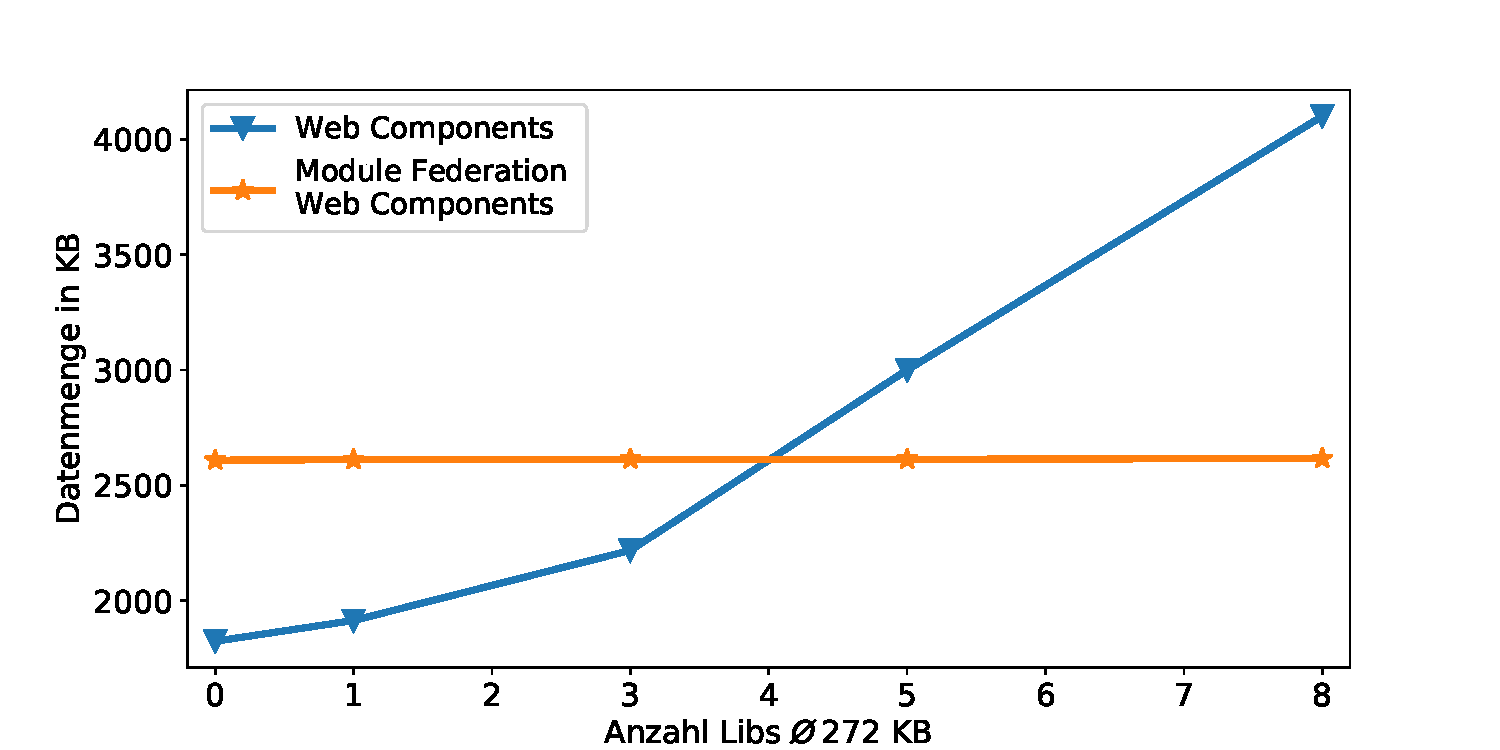
\includegraphics[width=1\textwidth]{img/appendix/DatasizeEval/MFWCvsMF_Datasize}}\\ % Pfad
		\source{Eigene Darstellung} % Quelle
		\label{fig:DatenmengeMFWC-WC}
	\end{minipage}
\end{figure}

Es wurden 5 Messungen mit null, einer, drei, fünf und acht verwendeten Bibliotheken durchgeführt. In \cref{fig:GGMessungBibs} in Anhang \ref{app:Bilder} sind die Bibliotheken pro Messlauf mit der durchschnittlichen Paketgröße dargestellt. Die vorherige \cref{fig:DatenmengeMFWC-WC} zeigt, dass ab 800\gls{KB}, welche durch Bibliotheken übertragen werden, Module Federation die bessere Art der Einbindung ist, um übertragene Datenmengen einzusparen. Die blaue Linie der Web Components Datenmenge weist einen leichten Knick am dritten Messpunkt auf, weil die eingebundenen Bibliotheken nicht alle genau dem Durchschnitt entsprechen.\footnote{Vgl. \cref{fig:GGMessungBibs} in Anhang \ref{app:Bilder}} Wären sie alle gleich groß, so würde der Graph linear verlaufen.

Allerdings ist das Teilen von Bibliotheken nur von Vorteil, wenn die Bibliothek ohnehin schon von der Portalshell geladen werden musste. Dies ist beispielsweise bei Standardbibliotheken wie \textit{@angular/core} oder einer geteilten Fachbibliothek, welche sowohl Microfrontend als auch die Portalshell benötigen, der Fall. Ebenfalls ist es auch vorstellbar, dass mehrere Microfrontends die gleiche Bibliothek benötigen, die Portalshell aber ursprünglich nicht. Dann könnte die Portalshell so umgebaut werden, dass die mehrfach benötigten Bibliotheken einmalig von der Portalshell eingebunden werden und sämtliche Microfrontends dann auf die eine eingebundene Bibliothek zugreifen, um Datenmenge zu sparen.

Module Federation kann gegenüber Web Components oder einem Iframe Vorteile bei der übertragenen Datenmenge bringen, jedoch nur im besonderen Anwendungsfall. Bei kleinen Microfrontends ohne abhängigen Bibliotheken sind Iframes und Web Components im Vorteil. Bei großen Lösungen mit vielen Bibliotheken, lohnt sich die Einbindung über Module Federation wiederum.

Das Kriterium \textit{Datenmenge} mit einer Gewichtung von 1,52\% wird daher mit 4 von 5 Punkten bewertet und erhält somit einen Teilnutzwert von 0,0608.

\textbf{Zwischenfazit}\\
Module Federation mit Web Components überträgt die Vorteile der Module Federation Einbindung von Angular Modulen auf andere Web Frameworks. Dadurch ist die Kompatibilität gegenüber anderen Frameworks hoch. Ebenfalls positiv anzumerken sind geringe Renderingzeiten sowie die Reduzierung der übertragenen Datenmenge, besonders bei geeigneten Konstellationen. Module Federation mit Web Components hat von den vier verglichenen Arten der Einbindung den höchsten Einrichtungsaufwand und ist ebenfalls kein offiziell anerkannter Standard von Angular.

\subsection{Vergleich der Arten untereinander}\label{sec:VergleichDerArten}

In diesem Abschnitt werden die im vorherigen Kapitel \cref{sec:AnalyseVerschiedenerIntegrationsansaetze} festgestellten Ausprägungen für jedes Kriterium jeder Alternative miteinander verglichen, um somit die beste Lösung für jedes Kriterium festzustellen.

In der nachfolgenden \cref{fig:ErgebnisNWA} sind die einzelnen Teilnutzwerte je Art der Einbindung und Kriterium in einer Tabelle gegenübergestellt. Die Teilnutzwerte sind gruppiert pro Kriterium in einer Farbskala dargestellt, damit der höchste Teilnutzwert (in grün) je Kriterium erkennbar ist.

\newpage
\begin{figure}[hbt!]
	\begin{minipage}[t]{1\textwidth}	
		\caption{Gegenüberstellung Ergebnisse der Nutzwertanalyse}
		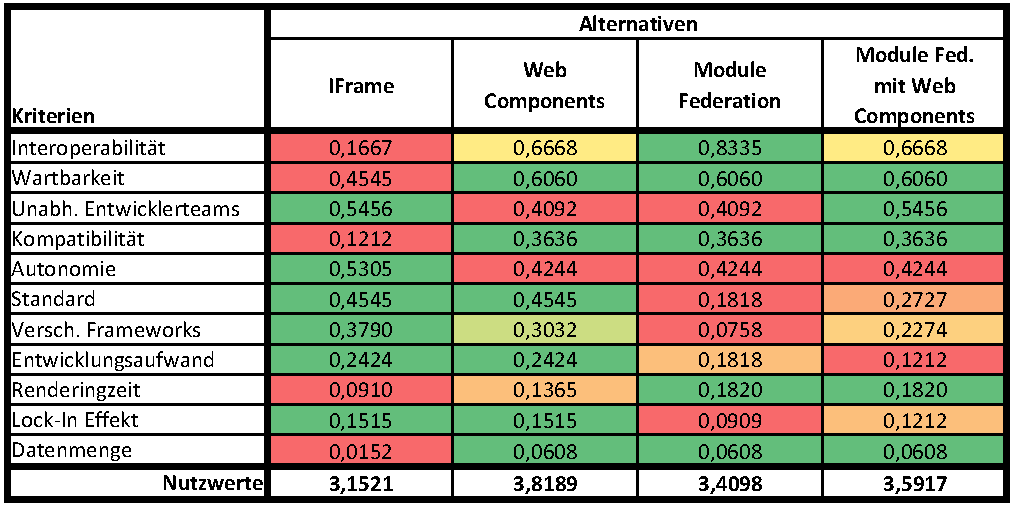
\includegraphics[width=1\textwidth]{img/ErgebnisNWA}\\ % Pfad
		\source{Eigene Darstellung} % Quelle
		\label{fig:ErgebnisNWA}
	\end{minipage}
\end{figure}

Für den gegebenen Anwendungsfall hat die Web Component bei der Evaluierung den höchsten Nutzwert erreicht. Dennoch konnten Web Components nicht bei allen Kriterien den höchsten Teilnutzwert erzielen, denn die direkte Gegenüberstellung der Einbindungsarten zeigt, dass keine der vier Arten für alle elf Kriterien am besten geeignet ist. 

Dies lässt darauf schließen, dass die Arten der Einbindung abhängig nach ihrem gegebenen Anwendungsfall optimal sind. Eine Übersicht, welche Art der Einbindung bei welchem Anwendungsfall optimal geeignet ist, wird im nachfolgenden \cref{sec:OptimaleAnwendungsszenarien} dargestellt.

\subsection{Optimale Anwendungsszenarien je nach Art der Einbindung}\label{sec:OptimaleAnwendungsszenarien}

In diesem Abschnitt werden Anwendungsszenarien mit den dazugehörigen Problemstellungen den Kriterien zugeteilt, danach mit den Arten der Einbindung verglichen und auf Basis der Ergebnisse ein Entscheidungsleitfaden gebildet.

Die nachfolgende \cref{tab:AnwendungsfallZuKriterium} zeigt vier Anwendungsfälle, welche verschiedene Problemstellungen aufweisen und dadurch unterschiedlich viel Wert auf einzelne Kriterien legen.

\begin{table}[!hbt]
	\centering
	\begin{minipage}[t]{1\textwidth}	
		\caption{Zusammenhang Kriterium zu Anwendungsfall} % Überschrift
		\begin{tabularx}{\columnwidth}{| c || X | c |}
			\toprule
			\thead{\textbf{Anwendungsfall}} & \thead{\textbf{Beispielhafte Problemstellung}} & \thead{\textbf{Kriterien}} \\
			\midrule
			Legacy Applikation & \makecell{Veraltete Frameworks,\\wenig KnowHow,\\keine Investition,\\Kundenanforderung} & \makecell{Entwicklungsaufwand,\\Kompatibilität} \\
			\midrule
			\makecell{Moderne Applikation,\\geringer Umfang} & \makecell{ReactJS als Framework,\\geringe Datenmenge nötig,\\Komplexität} & \makecell{Datenmenge,\\Frameworks}\\
			\midrule
			\makecell{Moderne Applikation,\\mittlerer Umfang}  & \makecell{Wiederverwendbar,\\Neuentwicklung, universell,\\Interoperabilität} & \makecell{Entwicklungsaufwand,\\Frameworks} \\
			\midrule
			\makecell{Moderne Applikation,\\großer Umfang} & \makecell{Angular als Framework,\\viel Routing,\\große Bibliotheken} & \makecell{Interoperabilität,\\Kompatibilität,\\ Datenmenge} \\
			\bottomrule
		\end{tabularx}
		\source{Eigene Darstellung}
		\label{tab:AnwendungsfallZuKriterium}
	\end{minipage}
\end{table}

Für vier Anwendungsfälle muss die jeweils beste Lösung zur Einbindung in die Portalshell gefunden werden. Dafür wird ein Entscheidungsbaum erstellt, welcher sich an dem von Geers im Grundlagenteil der Thesis in \cref{fig:EntscheidungsbaumArchitektur} orientiert, aber auf den Prototyp angepasst und durch die Erkenntnisse aus \cref{fig:ErgebnisNWA} optimiert ist. Der entwickelte Entscheidungsbaum ist in der nachfolgenden \cref{fig:Entscheidungsbaum} für Microfrontends zur Einbindung in eine Angular Portalapplikation dargestellt.

\newpage
\begin{figure}[hbt!]
	\centering
	\begin{minipage}[t]{0.95\textwidth}	
		\caption{Entscheidungsbaum: Einbindung Microfrontend in Portalshell}
		\frame{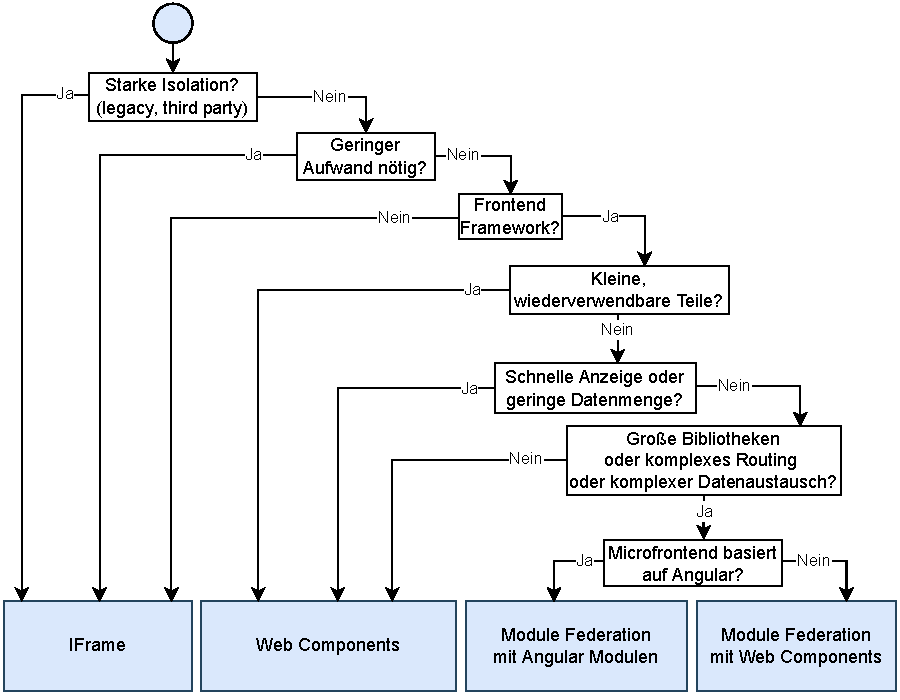
\includegraphics[width=1\textwidth]{img/Entscheidungsbaum}}\\ % Pfad
		\source{Eigene Darstellung} % Quelle
		\label{fig:Entscheidungsbaum}
	\end{minipage}
\end{figure}

Die Nutzwertanalyse hat ergeben, dass Iframes sich gut eignen, wenn Microfrontends eingebunden werden sollen, die Altlasten sind, nicht viel Aufwand erzeugen sollen, kein Web Frontend Framework enthalten oder stark gegen andere Microfrontends isoliert werden müssen. 

Ist der Use-Case des Microfrontends klein und wiederverwendbar, bspw. die konfigurierbaren Anzeige eines \gls{KPI}, oder kommt es auf schnelle Anzeige oder geringe übertragene Datenmenge bei wenig Bibliotheken an, so sind Web Components zu empfehlen.

Bei großer Datenmenge durch Bibliotheken, bei komplexem Routing im Microfrontend oder intensivem Datenaustausch mit der Portalshell empfiehlt sich die Einbindung über Module Federation. Abhängig davon, ob das Web Framework des Microfrontends Angular ist, sollte Module Federation mit Web Components oder mit Angular Modulen gewählt werden.